\documentclass[9pt]{article}
\usepackage[margin=2cm]{geometry}
\usepackage{booktabs,array,xspace,xcolor,longtable}
\usepackage{microtype}
\usepackage[section]{placeins}
\usepackage{tikz}
\usepackage{graphicx}
\graphicspath{{../Latex/figures/}}
% generated by make_assets_short.py - do not edit
\newcommand{\NCfg}{13}
\newcommand{\NExact}{12}
\newcommand{\NTcp}{14{,}200}
\newcommand{\NStageA}{5{,}200}
\newcommand{\NineShare}{35}
\newcommand{\NModelDiff}{25}
\newcommand{\NStageB}{9{,}000}
\newcommand{\CMaeZero}{0.30}
\newcommand{\CMaxZero}{0.7}
\newcommand{\CWrongZero}{0}
\newcommand{\CMaeOne}{7.39}
\newcommand{\CMaxOne}{99.4}
\newcommand{\CWrongOne}{2}
\newcommand{\CMaeTwo}{14.45}
\newcommand{\CMaxTwo}{99.4}
\newcommand{\CWrongTwo}{4}
\newcommand{\CMaeThree}{21.50}
\newcommand{\CMaxThree}{99.4}
\newcommand{\CWrongThree}{6}
\newcommand{\CN}{28}
\newcommand{\DN}{80}
\newcommand{\DDiff}{10}
\newcommand{\DJoinedWrongDiff}{10}
\newcommand{\DEarlyWrongDiff}{0}
\newcommand{\DJoinedMae}{17.8}
\newcommand{\DEarlyMae}{5.5}
\newcommand{\DJoinedWrong}{14}
\newcommand{\DEarlyWrong}{4}
\newcommand{\DBothWrong}{4}
\newcommand{\EFitEcdsa}{10}
\newcommand{\EFitMlFourFour}{12}
\newcommand{\EFitMlSixFive}{15}
\newcommand{\ECtlN}{36}
\newcommand{\ECtlMax}{0.9}
\newcommand{\ECtlWrong}{0}
\newcommand{\EN}{72}
\newcommand{\RJoinedMae}{1.42}
\newcommand{\RJoinedMax}{98.8}
\newcommand{\RJoinedWrong}{2}
\newcommand{\RJoinedRest}{142}
\newcommand{\RN}{144}
\newcommand{\RJoinedRestMax}{0.85}
\newcommand{\REarlyMae}{0.54}
\newcommand{\REarlyMax}{0.8}
\newcommand{\REarlyWrong}{0}
\newcommand{\REarlyRest}{144}
\newcommand{\RaceN}{221}
\newcommand{\RaceMlN}{134}
\newcommand{\RaceThr}{0.049}
\newcommand{\RaceRight}{132}
\newcommand{\RaceBeforePct}{90}
\newcommand{\RaceTwoRight}{36}
\newcommand{\RaceTwoScored}{36}
\newcommand{\RaceTwoOosRight}{394}
\newcommand{\RaceTwoOosN}{399}
\newcommand{\MixFitExc}{13}
\newcommand{\MixPredExc}{15}
\newcommand{\MixN}{4}
\newcommand{\MixRight}{3}
\newcommand{\NineDefMaeBefore}{13.3}
\newcommand{\NineDefMaeAfter}{1.2}
\newcommand{\NineN}{48}
\newcommand{\NineRwndDefOk}{7}
\newcommand{\NineRwndDefTot}{20}
\newcommand{\NineRwndLargeOk}{16}
\newcommand{\NineRwndLargeTot}{20}
\newcommand{\GenCells}{240}
\newcommand{\GenRespMax}{16}
\newcommand{\GenRttLo}{5}
\newcommand{\GenRttHi}{100}
\newcommand{\GenRateLo}{10}
\newcommand{\GenRateHi}{100}
\newcommand{\GenMtuLo}{1\,280}
\newcommand{\GenMtuHi}{9\,000}
\newcommand{\GenWEcRttFive}{10}
\newcommand{\GenWMFourFourRttFive}{10}
\newcommand{\GenWMSixFiveRttFive}{10}
\newcommand{\GenWEcRttThirty}{10}
\newcommand{\GenWMFourFourRttThirty}{12}
\newcommand{\GenWMSixFiveRttThirty}{15}
\newcommand{\GenWEcSlowTen}{10}
\newcommand{\GenWMFourFourSlowTen}{10}
\newcommand{\GenWMSixFiveSlowTen}{10}
\newcommand{\GenWEcMtuLow}{10}
\newcommand{\GenWMFourFourMtuLow}{12}
\newcommand{\GenWMSixFiveMtuLow}{16}
\newcommand{\ServCells}{48}
\newcommand{\ServWindow}{10}
\newcommand{\ServWrong}{0}
\newcommand{\BkN}{664}
\newcommand{\BkDef}{235}
\newcommand{\BkAOne}{44}
\newcommand{\BkAPct}{23.0}
\newcommand{\BkBRight}{248}
\newcommand{\BkBPct}{57.8}
\newcommand{\NtkRight}{18}
\newcommand{\NtkCells}{18}
\newcommand{\NtkEffect}{7}
\newcommand{\NtkEffectOk}{7}
\newcommand{\HN}{331}
\newcommand{\HLate}{117}
\newcommand{\HEarly}{214}
\newcommand{\HLateSS}{117}
\newcommand{\HWaitMed}{13.7}
\newcommand{\HEarlySS}{19}
\newcommand{\HAOne}{6}
\newcommand{\HALate}{117}
\newcommand{\HAPct}{5.1}
\newcommand{\HEnqMed}{181.2}
\newcommand{\HPcapMed}{-0.073}
\newcommand{\PhAfter}{164}
\newcommand{\PhAfterSS}{164}
\newcommand{\PhBefore}{500}
\newcommand{\PhBeforeSS}{61}
\newcommand{\StN}{799}
\newcommand{\StPOneRight}{799}
\newcommand{\StPOneN}{799}
\newcommand{\StPOnePct}{100.0}
\newcommand{\StPTwoRight}{212}
\newcommand{\StPTwoN}{236}
\newcommand{\StPTwoPct}{89.8}
\newcommand{\StPThreeRight}{51}
\newcommand{\StPThreeN}{74}
\newcommand{\StPThreePct}{68.9}
\newcommand{\StPTwoBRight}{236}
\newcommand{\StPTwoBN}{236}
\newcommand{\StDeferred}{71}
\newcommand{\StDeferredN}{96}
\newcommand{\StLate}{204}
\newcommand{\StLateInflight}{179}
\newcommand{\StLateLimited}{182}
\newcommand{\StEarly}{595}
\newcommand{\StEarlyLimited}{13}
\newcommand{\StBeforeN}{570}
\newcommand{\StBeforePk}{1}
\newcommand{\StAfterN}{204}
\newcommand{\StAfterPk}{10}
\newcommand{\KerN}{288}
\newcommand{\KerBeforeN}{216}
\newcommand{\KerBeforeSS}{0}
\newcommand{\KerAfterN}{72}
\newcommand{\KerAfterSS}{47}
\newcommand{\KerRight}{274}
\newcommand{\KerPct}{95.1}
\newcommand{\KerWrong}{14}
\newcommand{\KerMissLo}{0.039}
\newcommand{\KerMissHi}{0.080}
\newcommand{\KerMissNear}{0.031}
\newcommand{\AblFixedMae}{2.30}
\newcommand{\AblFixedOff}{4}
\newcommand{\AblFixedN}{144}
\newcommand{\AblSlowMae}{1.42}
\newcommand{\AblSlowOff}{2}
\newcommand{\AblSlowN}{144}
\newcommand{\AblLinuxMae}{1.42}
\newcommand{\AblLinuxOff}{2}
\newcommand{\AblLinuxN}{144}
\newcommand{\AblJoinedMae}{1.42}
\newcommand{\AblJoinedOff}{2}
\newcommand{\AblJoinedN}{144}
\newcommand{\AblEarlyMae}{0.54}
\newcommand{\AblEarlyOff}{0}
\newcommand{\AblEarlyN}{144}
\newcommand{\AblCFixedMae}{25.04}
\newcommand{\AblCFixedOff}{7}
\newcommand{\AblCFixedN}{28}
\newcommand{\AblCSlowMae}{35.63}
\newcommand{\AblCSlowOff}{10}
\newcommand{\AblCSlowN}{28}
\newcommand{\AblCLinuxMae}{0.30}
\newcommand{\AblCLinuxOff}{0}
\newcommand{\AblCLinuxN}{28}
\newcommand{\OvTwoSame}{247}
\newcommand{\OvTwoAll}{252}
\newcommand{\OvThreeSame}{247}
\newcommand{\OvThreeAll}{252}
\newcommand{\OvFourSame}{236}
\newcommand{\OvFourAll}{252}
\newcommand{\GxBaseCWrong}{0}
\newcommand{\GxBaseCLoose}{4}
\newcommand{\GxBaseDisEarly}{0}
\newcommand{\GxBaseDisJoined}{10}
\newcommand{\GxBaseEarlyWrong}{4}
\newcommand{\GxBaseMet}{4}
\newcommand{\GxFourCWrong}{0}
\newcommand{\GxFourCLoose}{4}
\newcommand{\GxFourDisEarly}{0}
\newcommand{\GxFourDisJoined}{10}
\newcommand{\GxFourEarlyWrong}{4}
\newcommand{\GxFourMet}{4}
\newcommand{\GxThreeCWrong}{0}
\newcommand{\GxThreeCLoose}{4}
\newcommand{\GxThreeDisEarly}{0}
\newcommand{\GxThreeDisJoined}{10}
\newcommand{\GxThreeEarlyWrong}{4}
\newcommand{\GxThreeMet}{4}
\newcommand{\GxMaxDiff}{0.05}
\newcommand{\CiWinLo}{64.0}
\newcommand{\CiWinHi}{99.8}
\newcommand{\CiJoinedLo}{95.1}
\newcommand{\CiJoinedHi}{99.8}
\newcommand{\CiRaceLo}{94.7}
\newcommand{\CiRaceHi}{99.8}
\newcommand{\CiKerLo}{92.0}
\newcommand{\CiKerHi}{97.3}
\newcommand{\CiNtkEffLo}{59.0}
\newcommand{\CiNtkEffHi}{100.0}
\newcommand{\SignDP}{0.002}
\newcommand{\SignNtkP}{0.016}

\newcommand{\GnineCellRows}{10 & ML-DSA-44 & 80 & 15\,635 / 17\,491 & 400 & \textbf{321} & 401 & 404 & 404 & 402\\
32 & ML-DSA-44 & 200 & 14\,394 / 17\,088 & 1001 & \textbf{803} & \textbf{803} & \textbf{803} & 1005 & \textbf{802}\\
56 & ECDSA-P256 & 150 & 3\,203 / 11\,150 & 600 & \textbf{451} & \textbf{451} & \textbf{452} & \textbf{452} & \textbf{450}\\
66 & ML-DSA-65 & 80 & 16\,685 / 16\,803 & 401 & \textbf{323} & \textbf{323} & \textbf{325} & 405 & \textbf{323}\\
72 & ML-DSA-87 & 200 & 20\,722 / 15\,294 & 1001 & \textbf{803} & \textbf{803} & \textbf{804} & \textbf{805} & \textbf{803}\\}

\newcommand{\OsRows}{client window (rule 1), 28 cells & 5 & 140 & 0 & 0\\
ticket timing, 80 cells & 5 & 400 & 0 & 14\\
ticket timing on new cells (G12, RTT 30 and 200) & 4 & 304 & 0 & 4\\
client window, delayed ACK (G14) & 4 & 112 & 0 & 0\\
ticket timing, delayed ACK (G14) & 4 & 128 & 0 & 0\\
ticket timing under BBR (G14) (not in the total) & 2 & 82 & 4 & 2\\
client window (rule 1), real link (G13-lite) & 1 & 28 & 0 & 0\\
ticket timing, real link (G13-lite) & 1 & 32 & 0 & 0\\
background load L0 (G17) & 1 & 22 & 0 & 0\\
background load L1 (G17) & 1 & 22 & 0 & 0\\
background load L2 (G17) & 1 & 22 & 0 & 0\\
background load L3 (G17) & 1 & 22 & 0 & 0\\
100 random cells (G19) & 5 & 500 & 0 & 19\\}

\newcommand{\StageARows}{base (the reference configuration) & 10 & 20 & 400 & 20\\
RTT 30 ms & 10 & 20 & 400 & 20\\
RTT 5 ms & 10 & 20 & 400 & 20\\
10 Mbit/s & 10 & 20 & 400 & 20\\
1 Gbit/s & 10 & 20 & 400 & 20\\
MTU 1\,280 & 10 & 20 & 400 & 20\\
MTU 9\,000 & 10 & 20 & 400 & 7\\
initial window 4 & 4 & 20 & 400 & 20\\
initial window 20 & 20 & 20 & 400 & 20\\
delayed ACK & 10 & 20 & 400 & 20\\
Cubic & 10 & 20 & 400 & 20\\
offload (TSO, GSO, GRO) & 10 & 20 & 400 & 20\\
TCP timestamps & 10 & 20 & 400 & 20\\}
\newcommand{\OffRows}{9 & ML-DSA-87 & 100 & 10 & 1\,280 & 14\,448 / 8\,919 & +9.8\\
79 & ML-DSA-87 & 30 & 10 & 1\,280 & 11\,121 / 3\,885 & +7.0\\
65 & ML-DSA-44 & 20 & 10 & 1\,280 & 20\,654 / 14\,985 & $-$4.9\\
54 & ML-DSA-87 & 50 & 10 & 1\,400 & 8\,498 / 5\,827 & +4.5\\
50 & ML-DSA-65 & 200 & 10 & 1\,500 & 8\,153 / 6\,812 & +4.5\\
38 & ML-DSA-65 & 100 & 10 & 1\,500 & 8\,095 / 16\,771 & +4.1\\
18 & ML-DSA-44 & 150 & 10 & 1\,280 & 19\,424 / 8\,436 & $-$3.6\\
28 & ML-DSA-44 & 80 & 10 & 1\,500 & 6\,491 / 8\,713 & +2.9\\
37 & ECDSA-P256 & 30 & 10 & 1\,400 & 17\,653 / 15\,197 & $-$2.6\\
48 & ML-DSA-44 & 30 & 10 & 1\,400 & 409 / 15\,258 & $-$2.1\\}
\newcommand{\TailRows}{ECDSA-P256 & 302 / 222 & 1\,000 & 302.3 & 302.6 & 303.9 & 303.9 & 0.00\\
ML-DSA-44 & 14\,500 / 12\,100 & 1\,000 & 403.8 & 404.0 & 406.2 & 406.2 & 0.00\\
ML-DSA-65 & 14\,500 / 12\,100 & 1\,000 & 403.7 & 404.0 & 405.0 & 405.0 & 0.00\\
ML-DSA-65 & 19\,460 / 9\,380 & 1\,000 & 403.9 & 404.1 & 405.5 & 405.5 & 0.00\\
ML-DSA-87 & 19\,460 / 10\,820 & 1\,000 & 404.1 & 404.5 & 406.6 & 406.6 & 0.00\\
ML-DSA-44 & 19\,460 / 10\,820 & 1\,000 & 404.0 & 404.1 & 406.0 & 406.0 & 0.00\\}

\newcommand{\GtfRows}{10 & unexplained & ML-DSA-44 & 20 of 60 & 20 of 60 & 6 of 60\\
32 & unexplained & ML-DSA-44 & 60 of 60 & 33 of 60 & 27 of 60\\
66 & unexplained & ML-DSA-65 & 60 of 60 & 23 of 60 & 60 of 60\\
72 & unexplained & ML-DSA-87 & 60 of 60 & 60 of 60 & 60 of 60\\
15 & never wrong & ECDSA-P256 & 0 of 60 & 0 of 60 & 0 of 60\\
16 & never wrong & ML-DSA-44 & 0 of 60 & 5 of 60 & 0 of 60\\
20 & never wrong & ECDSA-P256 & 0 of 60 & 0 of 60 & 0 of 60\\
37 & never wrong & ECDSA-P256 & 0 of 60 & 0 of 60 & 0 of 60\\
65 & never wrong & ML-DSA-44 & 0 of 60 & 0 of 60 & 0 of 60\\}

\newcommand{\pending}[1]{{\color{red}\textit{[pending: #1]}}}
\newcommand{\ms}{\,ms\xspace}
\renewcommand{\cite}[1]{[#1]}
\title{Supplement to ``Short Flights, Session Tickets, and the Linux TCP Window in Post-Quantum TLS Resumption''}
\author{Trong-Hieu Dinh \and Trong-Minh Hoang}
\date{}
\begin{document}
\maketitle
This supplement follows the order of the paper. First come the test populations, setups, and registered criteria; then the data behind the window rule (Section~4 of the paper) and the comparison of five models (Section~5). For the server window (Section~6) we give the evidence on how the kernel processes the ticket's acknowledgments (ACKs): the kernel's window test, a repeat with every event timed on one clock, and four rounds of interventions on the order of ACKs and the server's write; then the window in the random design points and the direction of the errors. The robustness tests follow, first on other machines (Section~7.1), then with other releases, libraries, controllers, load, and design points (Section~7.2). We close with smaller errors, what remains open, and the script behind each number (Table~\ref{tab:repro}). Machines are named as in Section~3 of the paper: X250 (Lenovo ThinkPad X250, Intel i7-5600U), OptiPlex (Dell OptiPlex 7460, Intel i7-8700), i9 (a workstation with an Intel i9-10900K), and GX10 (ASUS Ascent GX10, Arm Cortex-X925 and A725); all but the GX10 are x86-64, and the GX10 and the i9 are shared laboratory machines. The script \texttt{make\_assets\_short.py} generates most numbers from the archive; the rest are copied from the analysis outputs and design files named in the text. For the ticket ACK tests (Tests 6 to 12 and 27 of Table~2 of the paper), Table~\ref{tab:pop} gives the populations and kinds of evidence, Table~\ref{tab:setup} the setups, and Table~\ref{tab:crit} the registered criteria and outcomes. Criteria of the other registered tests are in Table~\ref{tab:crit2}. Not all evidence weighs the same, so we keep three kinds apart: a \emph{registered} test (its criterion was committed before the run, and a failure is reported as such), an \emph{intervention} (we change something on purpose), and a \emph{post hoc} reading (made after seeing the data, which can suggest but not confirm).

\section*{Tests, setups, and criteria (Section~3 of the paper)}
\emph{Scope and terms.} The paper asks how far Linux enlarges the congestion window after a short flight; why two resumed configurations needed one round-trip time (RTT) less than predicted; and what enlarges the server's window after the session ticket, and in which direction a model errs that ignores the enlargement. Its TLS results concern resumed connections with mutual authentication, since only there does the ticket carry a certificate chain, which with ML-DSA spans several segments. Under server-only authentication the ticket fits in one segment, and the server's window stays at \ServWindow\ segments (Section~6 of the paper). Throughout, ``window'' means the sender's congestion window (\texttt{snd\_cwnd}, in segments). A server's \emph{burst}, a word that recurs below, is the number of response segments it sends before the first ACK of the response can return, in other words the window it actually used. A \emph{discriminating} design point is one where the predictions of two models differ by more than half an RTT. A design point is \emph{wrong} (``mispredicted'' in the paper) when a prediction is off by more than that.

The ticket ACK tests (Table~\ref{tab:pop}) are not a single sample. Their units differ, and they come from separate runs.

\begin{table}[h]
\caption{Populations of the tests.}
\label{tab:pop}
\centering\footnotesize\setlength{\tabcolsep}{4pt}
\begin{tabular}{@{}p{0.17\textwidth}p{0.13\textwidth}p{0.065\textwidth}p{0.20\textwidth}p{0.26\textwidth}@{}}
\toprule
Test & Unit & Size & Evidence & Used for\\
\midrule
Captures of the server's link & transaction & \RaceN & the rule was found on these (post hoc) & order of the ticket's acknowledgments and the response (\RaceMlN\ with ML-DSA)\\
Request-size sweep & design point / transaction & \RaceTwoScored\ / \RaceTwoOosN & registered, met & the rule against the burst; the \RaceTwoScored\ design points are those outside the borderline band\\
Function trace & acknowledgment & \KerN & registered, met & \texttt{tcp\_slow\_start} against the timing rule (\KerBeforeN\ before the last request segment, \KerAfterN\ after it)\\
State trace & acknowledgment & \StN & registered: one criterion met, two not; further readings post hoc & the kernel's own test against \texttt{tcp\_slow\_start}; \StPThreeN\ lie near the threshold\\
Socket backlog & acknowledgment & \BkN & registered, not met; further reading post hoc & ownership of the socket as the cause of the delay\\
Softirq queue & acknowledgment & \HN & registered, not met; timing post hoc & queueing as the cause; \HALate\ are late acknowledgments\\
Clock-safe repeat, race design & transaction & \RpKFourN & registered (K1--K7), clock fixed: K2, K4, K5 met, K1 not met; K6, a rule for the text, met; K3, K7 reported & time bases, the true send time of the server's segments, the share acknowledged before the write\\
Clock-safe repeat, softirq design & acknowledgment & \RpKFiveN & registered, as above & late acknowledgments against the first response segment\\
No-ticket intervention & design point & \NtkCells & intervention, registered, met & role of the ticket; \NtkEffect\ design points have a burst above ten with the ticket\\
\bottomrule
\end{tabular}
\end{table}

These tests ran on November 1 and 2, 2026, in the namespace testbed on the paper's main platform (Section~3), the X250, with the server on CPU~1 and the client on CPU~0. One exception: the clock-safe repeat of November 21, 2026, also ran on the OptiPlex and the GX10, and on November 26 on the i9. Table~\ref{tab:setup} writes the suites as ECDSA-P256 (E), ML-DSA-44 (M44) and ML-DSA-65 (M65) and gives networks as RTT in ms (at 100 Mbit/s and MTU 1500 unless stated), while $n$ is the number of resumed transactions per design point.

\begin{table}[h]
\caption{Setup of the tests.}
\label{tab:setup}
\centering\footnotesize\setlength{\tabcolsep}{4pt}
\begin{tabular}{@{}p{0.14\textwidth}p{0.36\textwidth}rp{0.35\textwidth}@{}}
\toprule
Test & Design points & $n$ & Probes\\
\midrule
Captures & E, M44, M65; ten networks (RTT 5, 10, 15, 20, 30, 50, 100; RTT 100 at 10 Mbit/s, at MTU 1280 and at 9\,000); request 19\,460\,B, response 13 segments & 8 & \texttt{tcpdump} on the server's link; tracepoint \texttt{tcp:tcp\_probe}\\
Request-size sweep & M44, M65; RTT 30 and 100; ten request sizes from 15\,140 to 28\,100\,B (steps of 1\,440\,B), response 16 segments (40 design points) & 10 & \texttt{tcpdump} on the server's link\\
Function trace & M44, M65; RTT 5 and 30; requests 19\,460 and 25\,220\,B; response 16 segments (8 design points) & 6 & function tracer on \texttt{tcp\_reno\_cong\_avoid}, \texttt{tcp\_slow\_start}, \texttt{tcp\_sendmsg}, \texttt{tcp\_rcv\_established}; \texttt{tcp\_probe}; capture\\
State trace & E, M44, M65; RTT 5, 30, 100; RTT 30 at 10 Mbit/s and at MTU 1280; the same two requests; response 16 segments & 6 & \texttt{bpftrace} kprobes on \texttt{tcp\_reno\_cong\_avoid} (\texttt{snd\_cwnd}, \texttt{snd\_ssthresh}, \texttt{packets\_out}, \texttt{max\_packets\_out}, \texttt{is\_cwnd\_limited}) and \texttt{tcp\_slow\_start}; capture\\
Socket backlog & E, M44, M65; RTT 30, 100; RTT 30 at MTU 1280; the same two requests (18 design points) & 10 & kprobes on \texttt{\_\_release\_sock}, \texttt{tcp\_sendmsg}, \texttt{tcp\_reno\_cong\_avoid}, \texttt{tcp\_slow\_start}; capture\\
Softirq queue & E, M44, M65; RTT 30, 100; request 19\,460\,B; response 16 segments & 15 & tracepoints \texttt{net:netif\_rx}, \texttt{irq:softirq\_entry/exit}, \texttt{sched:sched\_switch}; kprobes on \texttt{tcp\_v6\_rcv}, \texttt{tcp\_sendmsg}, \texttt{\_\_release\_sock} and the two Reno functions; capture. The server on CPU~3 was an exploratory second arm, not reported\\
Clock-safe repeat & the race design and the softirq design again, with the CPU clock fixed (performance governor, no turbo) and, as a first repeat, as the system leaves it & 8, 15 & \texttt{ticket\_xmit.bt} (XQ, XS, RX, the server's write) and the softirq probes with XQ and XS; \texttt{clock\_sync.py}; capture\\
No-ticket intervention & the 18 design points of the backlog run, with and without a ticket on resumed connections (\texttt{tls\_probe --no-resumed-ticket}) & 10 & capture\\
\bottomrule
\end{tabular}
\end{table}

Each criterion in Table~\ref{tab:crit} was fixed in a prediction file or analysis script committed before the run. Any caveat about commit order is recorded in the archive's pre-registration table (\texttt{PREREGISTRATION\_L1.md}).

\begin{table}[h]
\caption{Registered criteria and outcomes.}
\label{tab:crit}
\centering\footnotesize\setlength{\tabcolsep}{4pt}
\begin{tabular}{@{}p{0.13\textwidth}p{0.35\textwidth}p{0.30\textwidth}p{0.13\textwidth}@{}}
\toprule
Test & Criterion & Result & Outcome\\
\midrule
Captures & burst above ten occurs only when the ticket's acknowledgment arrives before the write, in at least 80\% & the ticket was acknowledged before the write in \RaceBeforePct\% of the transactions, windows of ten included (read on the capture's clock) & not supported\\
Sweep & at least 90\% of the scored design points right; first request size with a burst of ten within one segment (1\,440\,B) of the predicted one & \RaceTwoRight\ of \RaceTwoScored\ design points; within one segment in all four series & met\\
Function trace & at least 90\% of the acknowledgments classified by the rule & \KerRight\ of \KerN\ (\KerPct\%) & met\\
State, P1 & \texttt{tcp\_slow\_start} is called iff the kernel's own test holds, in at least 98\% & \StPOneRight\ of \StPOneN & met\\
State, P2 & burst equals the window at the write minus the ticket segments still unacknowledged, within one segment, in at least 90\% of the transactions & \StPTwoPct\% & not met\\
State, P3 & the 0.049\ms rule agrees with the state for at least 90\% of the acknowledgments within 0.1\ms of the threshold & \StPThreeRight\ of \StPThreeN\ (\StPThreePct\%) & not met\\
Backlog, G1a & of the acknowledgments that arrived before the write and called \texttt{tcp\_slow\_start}, at least 90\% were deferred to the backlog & \BkAPct\% & not met\\
Backlog, G1b & of those processed on arrival, at least 90\% did not call it & \BkBPct\% & not met\\
Softirq, H1a & at least 80\% of the late acknowledgments were queued before the write returned & \HAOne\ of \HALate\ (\HAPct\%) & not met\\
Softirq, H1b & of those, at least 80\% of the waits overlap the server running on the same CPU & \HBOne\ of \HBN & not met\\
Clock-safe repeat, K1, K2, K4, K5 & see Table~\ref{tab:clock}; counted over the three runs with the clock fixed: two on the X250 (the second under ``Run to run'') and one on the OptiPlex & K2 and K4 met in all three; K5 met in both X250 runs, untestable on the OptiPlex; K1 not met in any & 8 of 11 met\\
Clock-safe repeat, GX10, D1--D5 & K2 and K4 (D1), K5 (D2), burst above ten in at most 25\% (D3), the rule of 0.049\ms at 90\% (D4), K6 (D5) & D1: K2 \RgKTwoPct\%; D2: \RgKFiveRight\ of \RgKFiveN; D3: \RgKSevenPos\ of \RgKSevenN; D4: \RgKSevenRight\ of \RgKSevenN\ (\RgKSevenPct\%); D5: \RgKSixPct\% and \RgKSixSmallPct\% & 3 of 5 met\\
No ticket, G2a--c & burst of ten or less in at least 95\% of the transactions of every design point without a ticket (a); in the design points where the ticket gave a burst above ten in half or more, in all of them (b); median burst without a ticket not larger than with (c) & \NtkCells\ of \NtkCells\ design points (a); \NtkEffect\ of \NtkEffect\ (b); \NtkCells\ of \NtkCells\ (c) & met\\
\bottomrule
\end{tabular}
\end{table}

\FloatBarrier
For the paper's other registered tests (Tests 13 to 31 of its Table~2), Table~\ref{tab:crit2} lists the criteria, with the thresholds approved before each run. The paper reports the outcomes. Unless a test states otherwise, ``wrong'' means that a prediction is off by more than half an RTT.

\begin{footnotesize}
\begin{longtable}{@{}p{0.045\textwidth}p{0.20\textwidth}p{0.705\textwidth}@{}}
\caption{Criteria of the other registered tests (fixed before each run).}\label{tab:crit2}\\
\toprule
No. & Test & Criteria\\
\midrule
\endfirsthead
\toprule
No. & Test & Criteria\\
\midrule
\endhead
\bottomrule
\endfoot
13 & OpenSSL 4.1.0 and 3.6.5, baseline 3.5 on the same machine & G1: rule~(1) wrong on at most 1 of the 28 client-window design points. G2: the rule loosened by two segments wrong on at least 3 of 28. G3: of the 10 design points where the two ticket models differ, the separate-ticket model wrong on at most 1 and the coalesced-ticket model on at least 9. G4: the separate-ticket model wrong on at most 6 of the 80 design points. The baseline must meet G1 to G4, or the other runs are inconclusive.\\
14 & Go \texttt{crypto/tls} & H1: rule~(1) wrong on at most 2 of 32 design points. H2: the loosened rule wrong on at least 2 of its 3 discriminating design points and textbook slow start on at least 4 of its 5. H3: of the 74 design points where the Go model and the coalesced-ticket model differ, the Go model wrong on at most 12. H4: wrong on at most 17 of the 114 design points. H5: at least 20 valid transactions per design point, and the bytes read by the client equal the calibrated flights (\textpm16\,B; it failed by the server's \GoClose-byte \texttt{close\_notify}, which the client also reads and the calibration lacks, and passes with that allowance, which was not registered). The ticket of Go is \GoTktLoKB\ to \GoTktHiKB\,KB.\\
15 & BBR and \texttt{fq} pacing, plain TCP & Q1: under BBR the window equals $w_0+n$ for at least 18 of the 20 sizes. Q2: under BBR rule~(1) is wrong for at least 8 of the 9 sizes $n\le 9$. Q3: with \texttt{fq} (Reno, Cubic) the window equals rule~(1) for at least 9 of the 10 sizes $n\le 10$. Q4: the burst time within 3\,ms of the unpaced baseline for at least 9 of those 10. Q5: the baseline has the window of rule~(1) for at least 18 of 20 sizes, or the other results are inconclusive. Q3 and Q4 count separately for Reno and Cubic, hence seven outcomes per machine.\\
16 & Ticket timing on new design points, RTT 30 and 200\,ms & Per RTT. K1: the separate-ticket model wrong on at most 2 of the 16 discriminating design points. K2: the coalesced-ticket model wrong on at least 14. K3: the separate-ticket model wrong on at most 8 of the 38 design points. K4: at least 30 valid transactions per design point.\\
17 & Client window and ticket timing under BBR & B1: the model with window $w_0+n$ wrong on at most 2 of the 28 client-window design points. B2: rule~(1) wrong on at least 8 of the 10 design points where it differs from $w_0+n$. B3: the BBR ticket model wrong on at most 8 of the 41 design points. B4: the model of the paper wrong on at least 17 of the 21 design points where it differs from the BBR model. B5: at least 30 valid transactions per design point.\\
18 & The same tests with delayed acknowledgments & D1: rule~(1) wrong on at most 2 of 28 design points. D2: the separate-ticket model wrong on at most 2 of the 10 discriminating design points. D3: the coalesced-ticket model wrong on at least 8 of the 10. D4: the separate-ticket model wrong on at most 7 of the 32 design points. D5: at least 30 valid transactions per design point.\\
19 & Window rule under loss, plain TCP & L1: per (loss, $n$) design point the share of connections whose window equals rule~(1) lies within 6 percentage points of $(1-p)^n$ in at least 24 of the 30 design points. L2: among the connections without a retransmission the window equals rule~(1) in at least 95\,\%. L3: at least 150 valid connections per design point.\\
20 & Random draw of 100 design points & R1: the separate-ticket model wrong on at most 3 of the 100 design points. R2: at least 85 design points within 2\,ms. R3: mean absolute error over the 100 design points at most 2\,ms. R4: at least 30 valid transactions per design point. R5: of the $D$ design points where the two ticket models differ, the separate-ticket model wrong on at most 10\,\% of $D$ and the coalesced-ticket model on at least 80\,\%.\\
21 & The three deviating BBR design points again ($n=200$) & S1: each within 5\,ms of its first value. S2: at least 190 valid shaped transactions each.\\
22 & Tails of six design points ($n=1\,000$) & T1: in every design point at most 1\,\% of the transactions exceed the median by more than 20\,ms. T2: at least 950 valid transactions per design point.\\
23 & Pipelined variant of the model for Go & P1: wrong on at most 4 of the 48 ML-DSA-87 design points. P2: the registered Go model wrong on at least 43 of the 48. P3: on the 12 ML-DSA-65 controls each prediction wrong on at most 1. P4: at least 30 valid transactions per design point.\\
24 & Background load, four levels & Y1: without load the model wrong on at most 1 of the 22 design points. Y2: at each loaded level on at most 3. Y3: at every level the coalesced-ticket model wrong on at least 8 of the 10 discriminating design points. Y4: at least 30 valid transactions per design point.\\
25 & Physical link between two machines & F1: plain TCP, in each of two configurations at least 18 of the 20 flight sizes have the median window of rule~(1). F2: at least 95\,\% of the connections have it. F3: at least 15 valid repetitions per design point. The TLS design points: D1 to D5 of Test 18.\\
26 & The ECDSA-P256 design point of Test 20 again and five neighboring design points & U1: the design point measured again ($n=200$) within 5\,ms of its first value (450.7\,ms). U2: the model with the measured ticket size right on all 6 design points. U3: the model with the ticket size of the random draw wrong on all 3 discriminating design points. U4: at least 190 valid transactions in the first design point and 95 in each other.\\
27 & Clock-safe repeat of Tests 7 to 11 & K1 to K7 and, for the GX10, D1 to D5: Table~\ref{tab:crit} and the section on the repeat.\\
28 & Random draw on the GX10, OptiPlex and i9 & A1: on each of these (the ``second machine'') the model wrong on at most 7 of the 100 design points (first X250 run: 5). A2: at least 4 of the design points wrong in the first X250 run wrong on the second machine too. A3: at most 2 design points wrong on the second machine that were right in the first X250 run. A4: at least 30 valid transactions per design point. For the X250 again: V1: at least 4 of the first run's wrong design points wrong again; V2: at most 2 new wrong design points; V3: data.\\
29 & Tests 16 and 18 on the same machines; Test 17 on the i9 & K1 to K4, D1 to D5 and B1 to B5 as in Tests 16, 18 and 17.\\
30 & Tests 1 to 5 on the GX10 and i9, OpenSSL~3.5 & G1 to G4 as in Test 13, applied to the run itself, which needs all 28, 80 and 10 design points.\\
31 & Server window in the nine random design points where it decides a round trip (60 transactions per design point and machine) & Q1: the window rule holds in at least 99.914\,\% of window events. Q2: burst $=\min(\mbox{window},\mbox{response segments})$ in at least 99.6\,\% of transactions. Q3a: ``fast'' and ``window $\ge$ response segments'' agree in at least 95\,\%. Q3b: of the fast transactions in the design points wrong in an earlier run (at least 10 needed), at least 90\,\% have such a window. Q4: in no design point with both classes does the request of the fast ones take half an RTT less. Q5: where $10+{}$ticket segments $<$ response segments, at most 1\,\% are fast. i9 only, from the post hoc script written before its data: S1 and S2 repeat Q3a and Q3b; S3: the client's first request round is never smaller than rule~(1) and larger in at most 5\,\%.\\
\end{longtable}
\end{footnotesize}

\section*{Congestion window after a short flight (Section~4)}
\emph{The 13 configurations of the window scan (Section~4).} Every configuration in Table~\ref{tab:stagea} was measured at the same 20 flight sizes ($n_1=1\dots16,20,24,31,40$), with 20 connections per size. A size ``matches'' when the median window after the flight equals rule~(1) for the configuration's initial window. Twelve configurations match at all 20 sizes. The exception is MTU 9\,000, where only 7 of 20 sizes match: the receive window limits the sender, \texttt{is\_cwnd\_limited} stays false, and the window does not grow.

\begin{table}[h]
\caption{Flight sizes at which the median window equals rule~(1), by configuration of the window scan.}
\label{tab:stagea}
\centering\footnotesize\setlength{\tabcolsep}{4pt}
\begin{tabular}{@{}lrrrr@{}}
\toprule
Configuration (one factor changed from the base) & $w_0$ & Sizes & Connections & Sizes matching\\
\midrule
\StageARows
\bottomrule
\end{tabular}
\end{table}

\section*{Session-ticket placement: what each part of the model adds (Section~5)}
Table~\ref{tab:ablation} gives, for five models, the mean absolute error (MAE, in ms) and the number of design points wrong by a round trip. The first row is the paper's IW model, in which every flight starts with $w_0$ segments; it uses the write pattern of OpenSSL with a coalesced ticket. The other rows start from textbook slow start and add one element each; on the resumed configurations, textbook slow start and the row with Linux validation use ideal segmentation, whereas all three client-window rows use the write pattern of OpenSSL. On the resumed configurations, adding the validation test and then the write pattern changes neither figure; only writing the ticket separately does. The validation test matters in the client-window test.

\begin{table}[h]
\caption{What each part of the model adds.}
\label{tab:ablation}
\centering\footnotesize\setlength{\tabcolsep}{4pt}
\begin{tabular}{@{}lrrrr@{}}
\toprule
 & \multicolumn{2}{c}{\AblFixedN\ resumed} & \multicolumn{2}{c}{\AblCFixedN\ client window}\\
Model & MAE & wrong & MAE & wrong\\
\midrule
Window fixed at $w_0$ (IW model) & \AblFixedMae & \AblFixedOff & \AblCFixedMae & \AblCFixedOff\\
Textbook slow-start model & \AblSlowMae & \AblSlowOff & \AblCSlowMae & \AblCSlowOff\\
+ Linux validation, rule (1) & \AblLinuxMae & \AblLinuxOff & \AblCLinuxMae & \AblCLinuxOff\\
+ OpenSSL write pattern (coalesced-ticket model) & \AblJoinedMae & \AblJoinedOff & --- & ---\\
+ ticket written separately (separate-ticket model) & \AblEarlyMae & \AblEarlyOff & --- & ---\\
\bottomrule
\end{tabular}
\end{table}

\section*{Server window: what the kernel tests (Section~6)}
An ACK grows the window only if, when it is processed, the sender counts as cwnd-limited: \texttt{tcp\_reno\_cong\_avoid()} calls \texttt{tcp\_slow\_start()} only if \texttt{tcp\_is\_cwnd\_limited()} holds (Section~4 of the paper). For the ticket's ACKs, then, timing is decisive. An ACK processed while the response is in flight (\texttt{packets\_out} near the window) counts. One processed before the response is written is different: it counts only if the ticket's own segments make the socket cwnd-limited, that is, if \texttt{snd\_cwnd} is below twice \texttt{max\_packets\_out}; with a window of ten, a ticket of six segments or more meets this condition and a shorter one does not. The tests below examine when the ticket's ACKs are processed and what that order does to the window.

\emph{Clocks.} Three times need comparing: when an ACK is on the server's link (the capture: \texttt{tcpdump} on the server's veth end, wall clock), when the application's write returns, and when the kernel processes the ACK (both from \texttt{bpftrace}, \texttt{nsecs}, monotonic clock). The capture timestamps a packet from the client on its arrival at the server, but a packet from the server only after the egress delay of \texttt{netem}, so the analysis shifts the latter back by half the nominal RTT. We combine four kernel runs with the capture. The function trace (\KerN\ acknowledgments) fixes the constant between the two clocks with one packet seen by both, so the misses below lie within \KerMissNear\ms of the threshold, about the precision of that alignment. The state and backlog traces join each acknowledgment to the capture by client port and acknowledgment number and compare only times of one clock, so they need no alignment. For the softirq run we went back and checked the alignment (post hoc, \texttt{analyze\_clock\_check.py}): the offset between the capture's arrival stamp and the \texttt{netif\_rx} time of the same acknowledgment (\ClkN\ acknowledgments) has a 5th to 95th percentile of \ClkLo\ to \ClkHi\,\textmu s around its file's median and a largest deviation of \ClkMax\,\textmu s. Client-to-server times are therefore accurate to a few tens of microseconds. The other direction is less accurate: with the offset of the same file, the first response segment appears \ClkWriteAbs\,\textmu s after the return of the write that sent it, which cannot happen, since that write returns only after sending it. The nominal RTT/2 must therefore be too small by about that amount, which is the order of the extra delay that \texttt{netem} adds (0.3\ms of RTT on this machine in calibration runs on November 15). On the capture of these first traces, the order of a client packet and a server packet is thus uncertain by about 0.26\ms, more than both the 0.049\ms threshold and the 0.07\ms discussed below.

Figure~\ref{fig:timeline} shows a late ticket ACK (one processed after the response write has returned) on both clocks, with the write's return at 0 (medians of the softirq run). On the \texttt{bpftrace} clock the ACK is queued \HEnqMed\,\textmu s after the write returns and processed \HWaitMed\,\textmu s later. The capture, aligned to \texttt{bpftrace} using the arrival timestamps of the client's segments (precision about 10\,\textmu s), places the first response segment after the write returns, the impossible order noted above. Trust the capture alone, and the ACK appears \HPcapMedAbsUs\,\textmu s before the response; on a single clock it follows the write. These traces do not record the true send time of the segment (red, dashed); the section ``Repeat with every event on one clock'' measures it.

\begin{figure}[h]
\centering
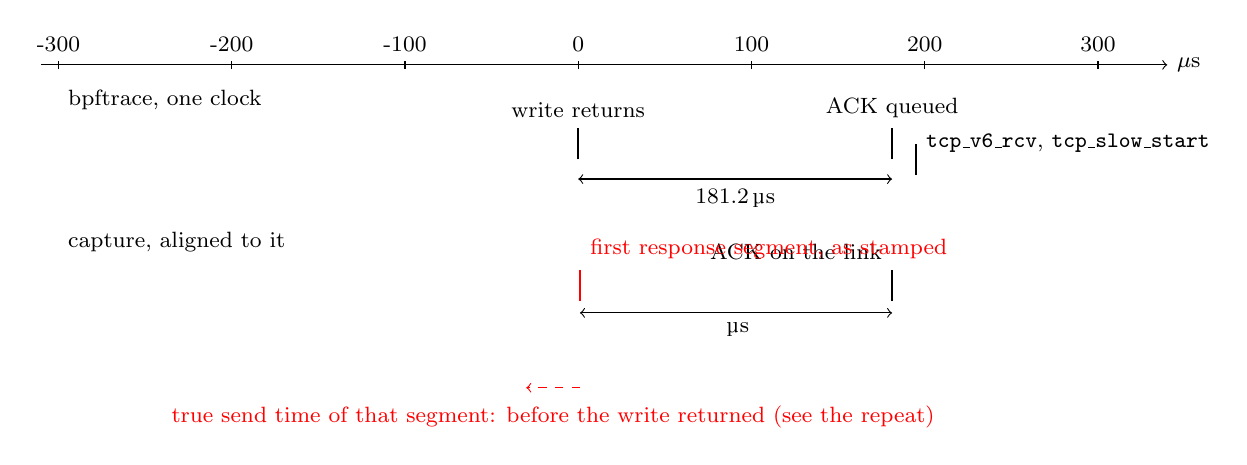
\begin{tikzpicture}[x=0.022cm, y=1cm, font=\footnotesize]
  \pgfmathsetmacro{\xe}{\HEnqMed}\pgfmathsetmacro{\xr}{\HEnqMed+\HWaitMed}\pgfmathsetmacro{\xs}{\ClkWriteAbs}
  \draw[->] (-310,2.2) -- (340,2.2) node[right] {$\mu$s};
  \foreach \t in {-300,-200,-100,0,100,200,300} {\draw (\t,2.15) -- (\t,2.25) node[above] {\t};}
  \node[anchor=west] at (-300,1.75) {bpftrace, one clock};
  \draw[thick] (0,1.0) -- (0,1.4) node[above] {write returns};
  \draw[thick] (\xe,1.0) -- (\xe,1.4) node[above] {ACK queued};
  \draw[thick] (\xr,0.8) -- (\xr,1.2) node[right] {\texttt{tcp\_v6\_rcv}, \texttt{tcp\_slow\_start}};
  \draw[<->] (0,0.75) -- node[below] {\HEnqMed\,\textmu s} (\xe,0.75);
  \node[anchor=west] at (-300,-0.05) {capture, aligned to it};
  \draw[thick] (\xe,-0.8) -- (\xe,-0.4) node[above left] {ACK on the link};
  \draw[thick,red] (\xs,-0.8) -- (\xs,-0.4) node[above right,red] {first response segment, as stamped};
  \draw[<->] (\xe,-0.95) -- node[below] {\HPcapMedAbsUs\,\textmu s} (\xs,-0.95);
  \draw[dashed,red,->] (\xs,-1.9) -- (-30,-1.9) node[midway,below=3pt,red] {true send time of that segment: before the write returned (see the repeat)};
\end{tikzpicture}
\caption{A late ticket ACK on two clocks.}
\label{fig:timeline}
\end{figure}

\emph{When the ACK counts.} An early ticket ACK does not, on its own, settle the window. In captures on the server's link (\RaceN\ resumed transactions, ten networks), at least one ticket segment is acknowledged before the response is written in \RaceBeforePct\% of the transactions, including some whose window stays at ten. This share comes from the capture clock, which orders client and server packets only to about a quarter of a millisecond; on one clock it is \RpKSixPct\% of \RpKSixN\ with the CPU clock fixed and \RuKSixPct\% of \RuKSixN\ with the clock left to the system (Table~\ref{tab:clock}). The arrival of the ticket's last ACK does a better job of separating the outcomes. We found this post hoc: the rule ``the window exceeds ten segments exactly when the last ACK arrives more than \RaceThr\ms after the last request segment'' is right on \RaceRight\ of \RaceMlN\ ML-DSA transactions in the run that produced it (exact 95\% interval \CiRaceLo--\CiRaceHi\%).

The rule then faced a request-size sweep with predictions committed beforehand, and held. Outside a borderline band (design points whose median lies within \RaceBand\ms of the threshold), \RaceTwoRight\ of \RaceTwoScored\ design points fell in the predicted class (95\% Wilson interval [90, 100]\%), and the rule classified \RaceTwoOosRight\ of \RaceTwoOosN\ transactions correctly ([97, 99.5]\%). Note what it predicts: whether the window grows, not how far. All small-request controls came out as predicted (\ECtlWrong\ of \ECtlN\ design points wrong). Table~\ref{tab:thr} gives the share of observations for which ``the ACK arrives more than $T$ after the last request segment'' agrees with the outcome. Because $T=\RaceThr$\ms was chosen on the first run, the table is post hoc; it shows that on this machine accuracy depends little on the exact threshold (\ThrSLoR--\ThrSHiR\% of transactions for $T$ from 0.04 to 0.10\ms, \ThrSA\% at 0.02\ms). With the CPU clock fixed, the rule carries over to the OptiPlex (next section). On the GX10, however, its agreement with the kernel's state falls short (Table~\ref{tab:repl} and the text with it).

\emph{What the kernel does.} A function trace of the server's kernel (criterion committed in the analysis script before the run) covers \KerN\ ticket ACKs. Reno examines every one, yet calls \texttt{tcp\_slow\_start} for none of the \KerBeforeN\ that arrive before the last request segment and for \KerAfterSS\% of the \KerAfterN\ that arrive after it. The timing rule classifies \KerRight\ of \KerN\ correctly (\KerPct\%; exact interval \CiKerLo--\CiKerHi\%). All \KerWrong\ misses lie within \KerMissNear\ms of the threshold, about the precision of the clock alignment.

A second run sidesteps the alignment problem by reading the sender's state at each ACK (\texttt{bpftrace} probes on both functions; \StN\ ACKs, matched to the capture by port and acknowledgment number). As registered (the paper's slow-start-condition test, called the state test below), \texttt{tcp\_\allowbreak slow\_\allowbreak start} is called iff the kernel's own test holds, that is, iff \texttt{is\_\allowbreak cwnd\_\allowbreak limited} is set or \texttt{snd\_\allowbreak cwnd} is below twice \texttt{max\_\allowbreak packets\_\allowbreak out} (\StPOneRight\ of \StPOneN). Two other registered criteria did not fare as well (P2 and P3 in Table~\ref{tab:crit} were not met). Because of P3, agreement between the timing rule and the kernel's state near the threshold, we treat the rule as a proxy, not the mechanism, and not as a constant of Linux TCP.

Post hoc, \StLateInflight\ of the \StLate\ ACKs that arrive more than \RaceThr\ms after the last request segment are processed with the response already in flight, where the test holds (median \texttt{packets\_out} \StAfterPk, against \StBeforePk\ for the others). Of the \StEarly\ ACKs that arrive no more than \RaceThr\ms after it, \StEarlyLimited\ find the sender limited; all are ML-DSA-65, where \texttt{max\_packets\_out} reaches six and $10<2\times6$. We cannot explain a third group, subject to the clock caveat above: the capture shows \StDeferredN\ ACKs arriving before the write but more than \RaceThr\ms after the last request segment, and \StDeferred\ of them are processed after the write. One more reading, again post hoc and distinct from the registered criterion P2, which failed: the burst equals the window after the last ticket ACK processed before the first ACK of the response (\StPTwoBRight\ of \StPTwoBN\ within one segment).

\emph{Why the ACKs are late, and the no-ticket intervention.} We had two explanations for the delay, and the data supported neither. The first was socket ownership (a third run, with probes on the socket backlog; \BkN\ ticket ACKs): only \BkDef\ were processed from the backlog, and both registered criteria failed (G1a and G1b in Table~\ref{tab:crit}). A post hoc look finds \texttt{tcp\_slow\_start} called for all \PhAfterSS\ ACKs processed after the first response write returned and for \PhBeforeSS\ of the \PhBefore\ processed before it, mostly in softirq context. The second explanation had the late ACKs waiting in the softirq queue (a fourth run, with probes on the enqueue to the per-CPU backlog, the receive path, and the softirq; \HN\ ticket ACKs). It failed its registered criteria too. Only \HAOne\ of the \HALate\ late ACKs had been queued before the write returned (H1a in Table~\ref{tab:crit}), and those waited only briefly for processing (median \HWaitMed\,\textmu s, on the same CPU). They were queued (post hoc) a median of \HEnqMed\,\textmu s after the write returned, although the capture places them 0.07\ms before it. The two orderings differ by \ClkDiff\,\textmu s, consistent with the clock uncertainty above, and we trust the kernel's own clock: these ACKs reached the server's input queue after the write had returned, which is why H1a failed.

One intervention does isolate the role of the ticket. Without a ticket on resumed connections, the burst stayed within ten segments in all \NtkCells\ design points, as predicted, including the \NtkEffect\ design points where the ticket pushes it above ten (exact sign test on those pairs, $p=\SignNtkP$).

\begin{table}[h]
\caption{Robustness of the ticket-timing rule to its threshold $T$ (post hoc).}
\label{tab:thr}
\centering\small
\begin{tabular*}{\columnwidth}{@{\extracolsep{\fill}}p{0.30\columnwidth}rrrrrr@{}}
\toprule
$T$ (ms) & 0.02 & 0.04 & 0.049 & 0.06 & 0.08 & 0.10\\
\midrule
Burst $>10$, \RaceTwoOosN\ transactions (\%) & \ThrSA & \ThrSB & \ThrSC & \ThrSD & \ThrSE & \ThrSF\\
\texttt{tcp\_slow\_start} called, \StN\ ACKs (\%) & \ThrFA & \ThrFB & \ThrFC & \ThrFD & \ThrFE & \ThrFF\\
\bottomrule
\end{tabular*}
\end{table}

\section*{Repeat with every event on one clock (Section~6)}
The clock check sent us back to repeat the traces on November 21, 2026, on the X250 and, with the CPU clock fixed, on the OptiPlex, with the procedure and criteria K1 to K7 fixed beforehand (\texttt{results/wp6\_pred\_clock.md}). This time, before each trace, \texttt{clock\_sync.py} records the offset between the wall clock and the monotonic clock and the state of the kernel clock, NTP (disabled for the run), and the CPU clock; after the trace it reads the offset again and rejects the file if the offset moved by more than 20\,\textmu s (\RpFiles\ of \RpFiles\ files passed). A new probe set, \texttt{ticket\_xmit.bt}, timestamps on the \texttt{bpftrace} clock when each segment of the connection is handed to the device (XQ), when it leaves the queueing discipline, where \texttt{tcpdump} stamps it (XS), when a segment arrives (RX), and when the server's write returns, so the true send time of the server's segments is now measured rather than inferred. The repeat reran the race design (30 files) and the softirq design (6 files) in two CPU states: first with the clock left to the system, then fixed (performance governor, no turbo) as in the first traces. Table~\ref{tab:clock} gives the outcomes.

\begin{table}[h]
\caption{Outcomes of the clock-safe repeat.}
\label{tab:clock}
\centering\footnotesize\setlength{\tabcolsep}{3pt}
\begin{tabular}{@{}p{0.24\textwidth}p{0.17\textwidth}p{0.17\textwidth}p{0.17\textwidth}p{0.14\textwidth}@{}}
\toprule
Criterion (fixed beforehand) & X250, CPU clock fixed & X250, clock as left & OptiPlex, clock fixed & Outcome (fixed)\\
\midrule
K1 arrival stamps equal RX: at least 95\% within 20\,\textmu s, all within 50\,\textmu s & \RpKOnePct\%, largest \RpKOneMax\,\textmu s & \RuKOnePct\%, largest \RuKOneMax\,\textmu s & \RoKOnePct\%, largest \RoKOneMax\,\textmu s & not met on both\\
K2 capture stamp of a server segment equals XS: at least 95\% within 20\,\textmu s & \RpKTwoPct\% (median $\RpKTwoMed$\,\textmu s) & \RuKTwoPct\% (median $\RuKTwoMed$\,\textmu s) & \RoKTwoPct\% (median $\RoKTwoMed$\,\textmu s) & met on both\\
K3 delay that the device adds beyond RTT/2, per direction (reported) & \RpKThreeLo\ to \RpKThreeHi\,\textmu s, median \RpKThreeMed & \RuKThreeLo\ to \RuKThreeHi\,\textmu s, median \RuKThreeMed & \RoKThreeLo\ to \RoKThreeHi\,\textmu s, median \RoKThreeMed & reported\\
K4 first response segment queued before the write returns: at least 99\% & \RpKFourRight\ of \RpKFourN & \RuKFourRight\ of \RuKFourN & \RoKFourRight\ of \RoKFourN & met on both\\
K5 late acknowledgments reach the queue after that segment: at least 90\% & \RpKFiveRight\ of \RpKFiveN & \RuKFiveRight\ of \RuKFiveN & \RoKFiveRight\ of \RoKFiveN\ (too few to test) & met; OptiPlex untested\\
K6 a ticket segment acknowledged before the write, overall and with a burst of ten or less, both at least 50\% (the statement in Section~6 stands) & \RpKSixPct\% of \RpKSixN; \RpKSixSmallPct\% of \RpKSixSmallN & \RuKSixPct\% of \RuKSixN; \RuKSixSmallPct\% of \RuKSixSmallN & \RoKSixPct\% of \RoKSixN; \RoKSixSmallPct\% of \RoKSixSmallN & met on both: statement stands\\
K7 rule of 0.049\ms on ML-DSA at MTU below 9\,000: transactions with a burst above ten, and the rule's accuracy (reported) & \RpKSevenPos\ of \RpKSevenN; \RpKSevenRight\ (\RpKSevenPct\%); best threshold \RpKSevenBestLo\ to \RpKSevenBestHi\ms & \RuKSevenPos\ of \RuKSevenN; \RuKSevenRight\ (\RuKSevenPct\%); best \RuKSevenBestLo\ms & \RoKSevenPos\ of \RoKSevenN; \RoKSevenRight\ (\RoKSevenPct\%); best \RoKSevenBestLo\ms & reported\\
\bottomrule
\end{tabular}
\end{table}

\emph{The clock.} For 90\% of the client's segments (5th to 95th percentile), the arrival timestamps agree with RX to within $\RpKOneLo$ to $+\RpKOneHi$\,\textmu s, with a tail reaching \RpKOneMax\,\textmu s. After removing a constant offset, the timestamps of the server's segments are within 20\,\textmu s of XS; \texttt{tcpdump} stamps a segment about \RpKTwoMed\,\textmu s from the tracepoint (negative: before it). Leave the CPU clock to the system, and the timestamps scatter more. The device adds about \RpKThreeMed\,\textmu s beyond half the nominal RTT in each direction, whereas the first analysis shifted the server's timestamps back by only the nominal half; this is of the same order as the 0.26\ms uncertainty of those traces.

\emph{The order.} On one clock, the first response segment is queued before its write returns in all \RpKFourN\ transactions, and all \RpKFiveN\ late ACKs reach the server's queue after that segment (K4 and K5). So the earlier impression from the capture, that the \emph{late} ACKs preceded the response, came from the capture's timestamps. The share of transactions with a ticket segment acknowledged before the response is written was \RaceBeforePct\% on the first run's capture; with every event on one clock it is \RpKSixPct\% of \RpKSixN\ (\RpKSixCapPct\% from the capture's own timestamps for the same transactions). The statement in Section~6 therefore stands, with the new percentage.

\emph{The CPU clock.} Then came a surprise. With the clock left to the system, the repeat did not reproduce the first traces. In ECDSA-P256 transactions the burst exceeded ten in \BuFirstEcUp\ of \BuFirstEcN\ in the first run, \BuPrEcUp\ of \BuPrEcN\ with the clock fixed (\BuPcEcUp\ of \BuPcEcN\ in a control with the first run's instruments), but \BuUrEcUp\ of \BuUrEcN\ with the clock left to the system (\BuUtEcUp\ of \BuUtEcN\ on repeating, and \BuUcEcUp\ of \BuUcEcN\ with the first run's instruments). The probes are therefore not the cause, and the control with the clock fixed reproduces the first traces (a criterion registered before it ran). To find the setting responsible, we separated two of them on the X250 (race design only). With the performance governor and turbo on (3.2 GHz), the ECDSA-P256 burst exceeded ten in \BuIsolAEcUp\ of \BuIsolAEcN\ transactions, as with the fixed clock, and the best threshold of the timing rule was \RaKSevenBestLo\ms. With the system's default governor (ondemand; idle cores at 500 MHz according to \texttt{clock\_sync.py}) and turbo off, it did so in \BuIsolBEcUp\ of \BuIsolBEcN, as with the clock left to the system, and the best threshold was \RbKSevenBestLo\ms (K1 \RbKOnePct\%, K2 \RbKTwoPct\%; \RbKSixPct\% of \RbKSixN\ transactions with a ticket segment acknowledged before the write). As predicted, the governor accounts for the difference and turbo does not; nothing else was varied. The best threshold depends on the clock in the same way. With the clock fixed, the unrefitted first-run threshold of 0.049\ms classifies \RpKSevenRight\ of \RpKSevenN\ transactions of the repeat correctly (\RpKSevenPct\%), and the best threshold on these data is \RpKSevenBestLo\ to \RpKSevenBestHi\ms. With the clock left to the system, 0.049\ms still classifies \RuKSevenRight\ of \RuKSevenN\ (\RuKSevenPct\%), but the best threshold moves to \RuKSevenBestLo\ms. The best threshold, in short, belongs to the machine's state, not to Linux TCP.

Figure~\ref{fig:k7} plots the underlying transactions. With the clock fixed, 0.049\ms (vertical line) parts the two groups. With turbo off, with the clock left to the system, and on the GX10, transactions with a burst above ten shift to the right and the groups overlap.

\begin{figure}[h]
\centering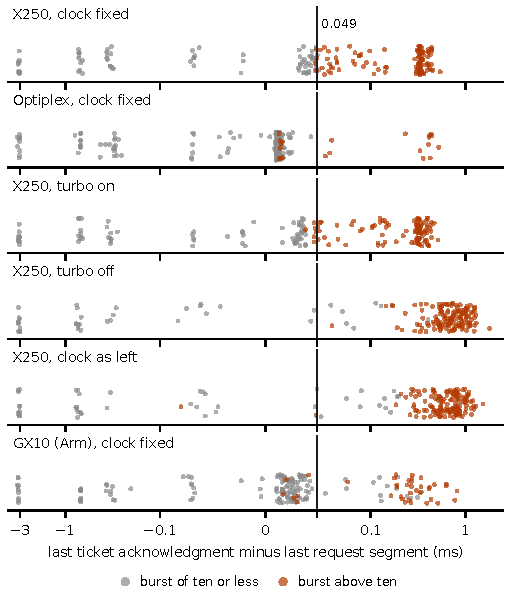
\includegraphics[width=0.62\textwidth]{fig_k7_points}
\caption{Each ML-DSA transaction at MTU below 9\,000, by the gap of its last ticket acknowledgment to the last request segment.}
\label{fig:k7}
\end{figure}

\emph{Run to run.} A second repeat on the X250 with the CPU clock fixed agrees with the first: K2 and K4 are met (\RqKTwoPct\%, \RqKFourRight\ of \RqKFourN), K5 is met (\RqKFiveRight\ of \RqKFiveN), K1 is not met again (\RqKOnePct\%), \RqKSixPct\% of \RqKSixN\ transactions have a ticket segment acknowledged before the write (against \RpKSixPct\%), and the rule of 0.049\ms classifies \RqKSevenRight\ of \RqKSevenN\ ML-DSA transactions (\RqKSevenPct\%, against \RpKSevenPct\%) with a best threshold of \RqKSevenBestLo\ms. The two runs satisfy the registered agreement criteria (within 5 points for the share and the accuracy, within 0.02\ms for the threshold), so we report these quantities as ranges over two runs.

\emph{The OptiPlex.} With Linux 7.0.0-42 and the CPU clock fixed, this machine gives similar clock results (Table~\ref{tab:clock}), except that the device adds more delay: about \RoKThreeMed\,\textmu s beyond RTT/2 at the longer RTTs against \RpKThreeMed\,\textmu s on the X250 (K3). A ticket segment is acknowledged before the write in \RoKSixPct\% of transactions (K6), so the statement in Section~6 holds on both machines with the CPU clock fixed. The sharp difference is how rarely the ticket enlarges the server's window there: of the \RoKSevenN\ ML-DSA transactions at MTU below 9\,000 the burst exceeds ten in \RoKSevenPos\ (\RpKSevenPos\ on the X250), so the softirq design gave too few late acknowledgments for K5 (\RoKFiveN). The rule of 0.049\ms still separates them, \RoKSevenRight\ of \RoKSevenN\ without refitting (\RoKSevenPct\%; the trivial answer, a burst of ten in every transaction, gets \the\numexpr\RoKSevenN-\RoKSevenPos\relax), and the best threshold is \RoKSevenBestLo\ms. We had predicted that the OptiPlex's best threshold would differ from the X250's by more than 0.02\ms. That prediction failed: it differs by \RoKSevenDiff\ms, and with the CPU clock fixed the threshold carried over to the OptiPlex.

\emph{The GX10.} Run as in its earlier traces (Linux 7.0.0-1025; client on CPU~0 and server on CPU~1; CPU clock reported as fixed: performance governor, no boost), the Arm machine met three of five registered predictions (D1 to D5). K4 holds (\RgKFourRight\ of \RgKFourN) and so does K5 (\RgKFiveRight\ of \RgKFiveN), the ticket enlarges the server's window rarely (a burst above ten in \RgKSevenPos\ of \RgKSevenN\ ML-DSA transactions at MTU below 9\,000, at most a quarter predicted), and \RgKSixPct\% of \RgKSixN\ transactions have a ticket segment acknowledged before the write (\RgKSixSmallPct\% of \RgKSixSmallN\ with a burst of ten or less). The other two fell short. K2 reached \RgKTwoPct\% within 20\,\textmu s (95\% required), and the rule of 0.049\ms classifies \RgKSevenRight\ of \RgKSevenN\ transactions (\RgKSevenPct\%; 90\% required; the trivial answer gets \the\numexpr\RgKSevenN-\RgKSevenPos\relax) with a best threshold of \RgKSevenBestLo\ms, against 0.047 to 0.048\ms on the X250 and 0.057\ms on the OptiPlex. K1 is not met either (\RgKOnePct\% within 20\,\textmu s, largest \RgKOneMax\,\textmu s), and the device adds \RgKThreeLo\ to \RgKThreeHi\,\textmu s beyond RTT/2. So even with every event on one clock, the threshold does not carry over to the GX10, which is the registered reading of D4. The statement in Section~6 holds (K6). The repeat did not rerun the state test, whose registered result stands.

\emph{The i9.} On November 26, 2026, we ran the repeat with the CPU clock fixed on the i9 (Linux 7.0.0-43; \texttt{results/wp6\_clock\_repeat\_i9\_analysis.txt}), with K1 to K7 unchanged. K1, K2, K4 and K5 were met. K1, not met on any earlier machine, holds here (100.0\,\% of 27\,166 segments within 20\,\textmu s, largest 24.6\,\textmu s), as does K2 (100.0\,\% of 14\,780 server segments within 20\,\textmu s); the first response segment is queued before its write returns in all 402 transactions (K4); and the 5 late ACKs, very few for a test, all reach the queue after that segment (K5). A ticket segment is acknowledged before the write in 90\,\% of 300 transactions (K6). The rule of 0.049\ms classifies 171 of 180 ML-DSA transactions (K7), but only 10 of them have a burst above ten, so that always answering ``ten or less'' is right on 170; the best threshold on these data is 0.477\ms. On the timing rule, then, the i9 offers little evidence.

\section*{The server's window, acknowledgment by acknowledgment (Section~6)}
If order matters, can we change it on purpose? Four rounds of experiments shift the order of ticket ACKs and the server's write. The first failed, which led to the second. The third moves the write instead of the ACKs, and the fourth is a registered confirmation of the third. The registered criteria are in the archive (\texttt{results/r3\_design.md} and the design and threshold files of rounds two to four); the numbers of round two come from \texttt{results/r3b\_report.txt}, those of rounds three and four from \texttt{r3c\_report.txt} and \texttt{r3d\_report.txt}.

\emph{Delaying the ACKs.} On the server's link, the client's pure ACKs (IPv6, TCP header only) are redirected to an \texttt{ifb} device whose \texttt{netem} qdisc delays them, and nothing else, by $\delta$ (0 to 1.6\,ms on the GX10, 0 to 6.4\,ms on the X250). On the kernel clock, the probe \texttt{ticket\_ack.bt} (\texttt{ticket\_ack2.bt} in the second round) records every \texttt{tcp\_ack} call on the server's socket and the socket state before and after it (in the second round also \texttt{max\_packets\_out}, \texttt{snd\_ssthresh}, and \texttt{is\_cwnd\_limited}). We ran the race design (request 25\,000\,B, RTT 100\,ms, 100\,Mbit/s, MTU 1\,500 and 1\,280, ECDSA-P256, ML-DSA-65 and -87, $n=30$, CPU clock fixed) at eight delays on the GX10 and seven on the X250.

\emph{First round: not supported.} The first-round criteria, registered on November 22, 2026, required that the shift of each ticket ACK follow $\delta$ within 20\,\textmu s (R1), that the burst equal the model's value for the transaction's own order (R2, 90\,\%), that the share of late ACKs rise with $\delta$ (R3), and that the ECDSA-P256 burst never exceed eleven (R4). R1 was not met (only 15.7\,\% of ticket ACKs on the GX10 and 55.6\,\% on the X250 complied: the medians follow $\delta$, but the spread far exceeds 20\,\textmu s), nor was R2 (\RbRoundThreeAMatch\,\% and \RbRoundThreeXMatch\,\%). R3 was formally met, on the X250 only because the order did not move. R4 failed on the GX10 (a burst of twelve in 79 of 488 transactions), because the delay affects every pure ACK, not only the ticket's. As registered, then, the round is not supported. It still taught us two things that shaped the second round: the burst is not a model constant, and we had set the criteria without knowing how widely our instrument scatters.

\emph{Second round.} A pilot on the GX10 (\RbPilotTxN\ transactions, \RbPilotEvN\ window events) fixed the thresholds by the rules in \texttt{r3b\_design.md}: a binomial band for the shares, as in Table~\ref{tab:gtls}, and twice the largest deviation of the median shift for the instrument. We committed them before opening any X250 data. The X250 run (\RbTestTxN\ transactions, \RbTestEvN\ window events) is the test.

\begin{table}[h]
\caption{Round two: the server's window read in the kernel (pilot on the GX10, test on the X250).}
\label{tab:rbtwo}
\centering\footnotesize\setlength{\tabcolsep}{4pt}
\begin{tabular}{@{}p{6.4cm}p{1.6cm}p{3.1cm}p{3.1cm}@{}}
\toprule
Criterion & Threshold & Pilot (GX10) & Test (X250)\\
\midrule
B1: \texttt{cwnd} after each ACK equals the slow-start rule, of events & 99.914\,\% & \RbPilotEvOk\ of \RbPilotEvN & \RbTestEvOk\ of \RbTestEvN\\
B2: burst $=\min(\texttt{cwnd},\ \mbox{segments of the response})$, of transactions & 99.6\,\% & \RbPilotTxOk\ of \RbPilotTxN & \RbTestTxOk\ of \RbTestTxN\\
B3: median shift follows $\delta$ within 47\,\textmu s; spread within $195+1.364\,\delta$ & & met & not met\\
B4: late share of the ML-DSA transactions (pooled) rises by 23.4 points or more per series from $\delta=0$ to the largest & & met (\RbPilotLateZero\ to \RbPilotLateMax\,\%) & not met (\RbTestLateZero\ to \RbTestLateMax\,\%)\\
B5: ECDSA-P256 with the accounting of B2 & 99.6\,\% & 512 of 512 & 448 of 448\\
B6: both machines meet B1 and B2, shares within 10 points & & & met\\
\bottomrule
\end{tabular}
\end{table}

\emph{What the second round shows.} (i)~In all \RbEvN\ window events on the two machines, the server's window follows the slow-start rule applied to the kernel's own counters (B1; because segments in the queue can span several MSS, the check counts acknowledged packets per MSS-sized piece). (ii)~In all \RbTxN\ of \RbTxN\ transactions, ECDSA-P256 included and with no fitted parameter, the response burst equals the smaller of the response size and the window left by the last ACK processed before the first ACK of the response can return. The thirteen-segment plateau that puzzled us in the first round turned out to be nothing but the response size. (iii)~The window after a ticket is therefore set by the number of ticket ACKs processed when the response is written, plus the late ones, each of which opens the window further while the response is being sent; a single rule covers both. (iv)~What causes the order, the round did not show. On the GX10 the delay changed it (the late share of ML-DSA transactions, pooled over the series, went from \RbPilotLateZero\,\% to \RbPilotLateMax\,\%); on the X250 it did not (B3 and B4 not met). There the 90th percentile of the shift follows $\delta$ (848, 1\,647, 3\,248, and 6\,447\,\textmu s at 0.8 to 6.4\,ms) while the 10th stays near 120\,\textmu s, so about half of the ticket ACKs are not delayed. The filter matches the same packets on both machines. Our hypothesis is that on the slower client many ticket ACKs are piggybacked on the request's data segments, which a pure-ACK filter misses. We did not test it. Fortunately, the third round does not depend on it, because it moves the other event, the write.

\emph{Third round: delaying the write.} The probe's server waits $D$ microseconds between the end of the request and the response (\texttt{tls\_probe --pre-write-delay-us}), and nothing else changes. A later write lets more ticket ACKs be processed before it, however they travel. The prediction uses only undelayed transactions. At delay $D$, a transaction counts as late if, at $D=0$, its last ticket ACK was processed more than the measured shift of the write after the write; the predicted late share at $D$ is the share of such transactions with the same suite and MTU. Nothing is fitted. The criteria (\texttt{results/r3c\_design.md}) were registered on November 23, 2026; their thresholds were derived from the GX10 pilot (\RcPilotTxN\ transactions, \RcPilotEvN\ window events) and committed before any X250 data were opened. Three definitions were fixed on the pilot (\texttt{r3c\_thresholds.md}): the use of the measured shift of the write instead of $D$, because the sleep timer adds about 60\,\textmu s on the GX10; the form of C2, because no pilot series had a 50\,\% late share at $D=0$; and the C1 tolerance of \RcTolerance\,\textmu s, which roughly allows for the timer overhead.

\begin{table}[h]
\caption{Third round: the write of the response delayed (test on the X250, delays 0 to \RcTestDMax\,\textmu s; the GX10 pilot for comparison).}
\label{tab:rcthree}
\centering\footnotesize\setlength{\tabcolsep}{4pt}
\begin{tabular}{@{}p{6.0cm}p{3.6cm}p{4.0cm}@{}}
\toprule
Criterion & Pilot (GX10) & Test (X250)\\
\midrule
C1: the median of $p_w$ moves by $D$ within \RcTolerance\,\textmu s (largest deviation) & met (\RcPilotDevMax\,\textmu s) & \textbf{not met} (\RcTestDevMax\,\textmu s, at the largest delay)\\
C2: the order moves in the predicted direction (ML-DSA-87: late share at $D=0$ and at the largest $D$) & met (\RcPilotLateZero\,\% to \RcPilotLateMax\,\%) & met (\RcTestLateZero\,\% to \RcTestLateMax\,\%)\\
C3: the late share is predicted from the $D=0$ transactions (design points within the band; mean absolute error against that of "no dependence on $D$") & met (\RcPilotCellsIn\ of \RcPilotCellsN; \RcPilotMeanErr\ against \RcPilotNullErr\ points) & \textbf{not met} (\RcTestCellsIn\ of \RcTestCellsN; \RcTestMeanErr\ against \RcTestNullErr\ points)\\
C4: the rule per window event; the burst accounting & \RcPilotEvOk\ of \RcPilotEvN; \RcPilotTxOk\ of \RcPilotTxN & \RcTestEvOk\ of \RcTestEvN; \RcTestTxOk\ of \RcTestTxN (met)\\
\bottomrule
\end{tabular}
\end{table}

Under the registered reading, because C1 was not met on the X250, no further conclusion is drawn there. The data do show why both were missed. The sleep adds 88 to 229\,\textmu s on the X250 (at most 7\,\% of $D$), against about 60 on the GX10. The one C3 design point outside its band (ML-DSA-87 at MTU~1\,500, $D=400$\,\textmu s: 9\,\% measured, 47\,\% predicted) lies where the distribution of undelayed ACK times is steep, so a small difference in the shift of the write changes the prediction a lot. Read as exploration rather than a test, the third round still shows on the X250 what the second could not: delaying the write moves the order in the predicted direction (the ML-DSA-87 late share falls from \RcTestLateZero\,\% to \RcTestLateMax\,\%), the undelayed transactions predict the late share in all design points but one, and the window rule and burst accounting hold (Table~\ref{tab:rcthree}).

\emph{Fourth round: a registered confirmation.} With the causes of the third round's two misses removed, we repeated the test on new data from both machines (\texttt{results/r3d\_design.md}, thresholds \texttt{r3d\_thresholds.md}, committed before the measurement). The server now busy-waits on the monotonic clock until the deadline (\texttt{--pre-write-spin-us}), which avoids timer slack. The prediction of the late share at delay $D$ now uses the full distribution of measured write shifts at $D$, not only their median; it still has no fitted parameter. Because it was defined after the third-round data were seen, those data are its training set (52 of 52 design points inside the band). Thresholds were derived from them by the rules in the design: the median of $p_w$ within 25\,\textmu s of $D$ (the floor for a spin-wait, a prediction that can fail); at most four of 28 to 36 design points outside the binomial band; a mean error of at most 5.2 points and at most 0.79 times that of ``no dependence on $D$''; and the second-round thresholds for the window rule and burst accounting.

\begin{table}[h]
\caption{Fourth round: the registered confirmation (write delayed by spinning; new data on both machines).}
\label{tab:rdfour}
\centering\footnotesize\setlength{\tabcolsep}{4pt}
\begin{tabular}{@{}p{6.0cm}p{3.6cm}p{4.0cm}@{}}
\toprule
Criterion & GX10 & X250\\
\midrule
C1: the median of $p_w$ moves by $D$ within 25\,\textmu s (deviations) & \textbf{not met} (\RdADevMin\ to \RdADevMax\,\textmu s; one level beyond 25) & met (\RdXDevMin\ to \RdXDevMax\,\textmu s)\\
C2: ML-DSA-87, late share from $D=0$ to the largest $D$ & met (\RdALateZero\,\% to \RdALateMax\,\%, both MTUs pooled) & met (\RdXLateZero\,\% to \RdXLateMax\,\%)\\
C3: design points inside the band; mean error against ``no dependence on $D$'' & \textbf{not met} (\RdACellsIn\ of \RdACellsN; \RdAMeanErr\ against \RdANullErr\ points) & met (\RdXCellsIn\ of \RdXCellsN; \RdXMeanErr\ against \RdXNullErr\ points)\\
C4: the rule per window event; the burst accounting & met (\RdAEvOk\ of \RdAEvN; \RdATxOk\ of \RdATxN) & met (\RdXEvOk\ of \RdXEvN; \RdXTxOk\ of \RdXTxN)\\
\bottomrule
\end{tabular}
\end{table}

\emph{Reading.} All four criteria were met on the X250 (Table~\ref{tab:rdfour}): the write moves by $D$ to within \RdXDevWorst\,\textmu s, and the order, shifted by the intervention, is predicted from unperturbed transactions. On the GX10 C2 and C4 were met, but C1 and C3 were not. The write moves by $D$ minus 15 to 30\,\textmu s, a systematic instrument shortfall that exceeds the registered 25\,\textmu s at one level. The ML-DSA-87 late share there is low at $D=0$ (\RdALateZero\,\%), and the no-dependence model fits better than the prediction (mean error \RdANullErr\ against \RdAMeanErr\ points). At intermediate delays, the late share of ML-DSA-87 rises above its value without delay (25 to 28\,\% at $D=150$ and 300\,\textmu s against 16 to 19\,\%) where the unperturbed times predict a fall. As registered, we draw no further conclusion for the GX10. We have not established why the share rises; the spinning server thread may disturb ACK processing there, but we did not test this. In short, the fourth round confirms the explanation to the registered criteria on the machine with a large late share, and confirms only its direction on the machine with a small one.

\emph{The fourth round on the i9.} We ran the same test with the same thresholds on the i9 on November 26, 2026 (1\,710 transactions; \texttt{results/r3d\_i9\_test.txt}; C5, which compares two machines, does not apply). C1 to C4 were met: the median shift of the write is within 17\,\textmu s of $D$; the late share does not rise; 31 of 32 design points lie in the band (mean error 2.6 points, against 3.6 for ``no dependence on $D$''); and the window rule and burst accounting hold in all 10\,225 events and 1\,710 transactions. The result carries limited weight: even without delay at most 9\,\% of the ML-DSA transactions are late, so C2 and C3 have little to distinguish. The one design point outside the band (ML-DSA-87, MTU 1280, $D=300$\,\textmu s: 53\,\% late, 6\,\% predicted) is a rise at an intermediate delay, as on the GX10, which we cannot explain.

\section*{The server's window in the random design points (Section~6)}
The wrong random design points carry a signature, and Test~31 (reported in Section~6 of the paper) measures what it suggests. We selected the design points by a rule that reads no measurement: every design point of the random draw in which a server window of 30 after an acknowledged ticket would change the prediction by more than half an RTT (nine of 100; \texttt{g24\_predict.py}). They contain the four wrong design points without a known cause (10, 32, 66 and 72; Table~\ref{tab:cells}, below, shows which design points each run got wrong) and five never wrong. Each machine measured two repetitions of 30 transactions per design point on the shaped link, with the CPU clock fixed, \texttt{ticket\_ack2.bt} and a capture, after an unshaped base run (\texttt{results/g24\_design.md}, registered on November 25, 2026, before any of these runs; the i9 criteria in an addendum, after the GX10 and X250 results). A transaction is \emph{fast} (``shortened'' in the paper) if its excess latency is below the midpoint of the two model values; its \emph{window} is the server's \texttt{snd\_cwnd} after the last ACK processed before the first ACK of the response can return. A response that leaves in one round needs a window at least its size, so that part of the agreement follows from how TCP sends; what the test adds is that the window, read independently of the latency, differs between fast and slow transactions of the same design point, and that the request side does not account for the saving.

\begin{table}[h]
\caption{Fast transactions, of 60 per design point and machine.}
\label{tab:gtf}
\centering\footnotesize\setlength{\tabcolsep}{4pt}
\begin{tabular}{@{}rllrrr@{}}
\toprule
Design point & In earlier runs & Suite & X250 & GX10 & i9\\
\midrule
\GtfRows
\bottomrule
\end{tabular}
\end{table}

\emph{Outcomes.} The registered criteria were met in \GtfXMet\ of \GtfXK\ on the X250, \GtfIMet\ of \GtfIK\ on the i9 (and S1 to S3), and \GtfGxMet\ of \GtfGxK\ on the GX10. Post hoc (\texttt{analyze\_g24\_posthoc.py}; registered on the i9), ``window $\ge$ response segments'' agrees with ``fast'' in \GtfXAgree\ of \GtfXW\ (X250), \GtfGxAgree\ of \GtfGxW\ (GX10) and \GtfIAgree\ of \GtfIW\ (i9) transactions with a window reading; over the three machines, \GtfUFastFit\ of \GtfUFast\ fast transactions of the four unexplained design points had such a window, and \GtfUSlowSmall\ of \GtfUSlow\ slow ones a smaller one. The client's first request round was never smaller than rule~(1) gives, and larger in \GtfXLarger, \GtfGxLarger\ and \GtfILarger\ of \GtfXN\ transactions each.

\emph{What did not go as registered, and limits.} (i)~Q5 failed on the GX10 on three transactions of design point 10, in which the registered script counted the 24-byte \texttt{close\_notify} as a fifteenth response segment; without it they agree, as do the other disagreements of Q3 on that machine. The registered output stands. (ii)~The registered script drops transactions when a client port is reused or the ticket leaves after the request; on the GX10 it dropped 10. Among them, five in design point 16 (never wrong) were fast by the \emph{request} side: the client sent the request in one round of 16 segments, against 12 or 14 otherwise, and Q4 would not be met with them included. We did not trace the client's window. On the GX10, none of the four design points without a known cause shows such a case. On the X250, one fast transaction of design point 72, one of the four, saved its round trip in the same way: the client sent the request in one round of 19 segments, against 18 as a rule, so the ticket left before the request was complete, the server's window stayed at ten, and the response took two rounds. It is the one fast transaction of these four design points without a window at least the size of the response. The i9 shows no such case. (iii)~The share of fast transactions varies between machines and between repetitions (design point 10: 18 then 2 of 30 on the GX10, 3 then 17 on the X250). The test shows which window goes with a fast transaction, not why the acknowledgments are processed early enough in only some of them. (iv)~The load of the GX10 during its run was low (\texttt{sar}: 1.7\,\% of CPU time in the interval within the run); that of the i9 was not recorded.

\section*{Direction of the errors (Section~6)}
With OpenSSL under Reno, the paper's model is off by more than half an RTT in \OsSlow\ of \OsRuns\ design-point runs, and in all \OsSlow\ of them it predicts a larger latency than measured; it is never too fast by that margin. This count was made after the measurements; for GnuTLS, the same direction was fixed beforehand (section on the third library, below). Table~\ref{tab:dir} counts the design-point runs of all tests with per-design-point predictions (client window, ticket timing, new design points, delayed ACKs, physical link, background load, and the random draw, on up to five machines or runs). Design points recur across runs (three OpenSSL releases, several machines): the \OsRuns\ design-point runs cover \OsCells\ design points, counting each once per test. The one-sidedness has a likely reason: the model gives the server a window of ten after the ticket, which the ticket can only enlarge. The count excludes loss, MTU 9\,000, Go, full handshakes, and BBR, whose window does not follow rule~(1). Under BBR, four design-point runs are too fast: on the X250 and on the i9, the two ML-DSA-87 design points that Section~7.2 places between the BBR and Reno predictions. With delayed ACKs the model underestimates by up to \OsMaxDelack\,ms, the delayed-ACK timer that it omits, which is less than half an RTT; elsewhere the largest underestimate is \OsMaxElse\,ms.

\begin{table}[h]
\caption{Design-point runs by direction of the error, with errors of more than half an RTT counted.}
\label{tab:dir}
\centering\footnotesize\setlength{\tabcolsep}{4pt}
\begin{tabular}{@{}lrrrr@{}}
\toprule
Test & Runs & Design-point runs & Too fast & Too slow\\
\midrule
\OsRows
\bottomrule
\end{tabular}
\end{table}

\section*{The same tests on other machines (Section~7.1)}
Would the random design points fail in the same places elsewhere? On November 21, 2026, we measured the paper's random design (Test 20 of its Table~2) in three more runs with criteria fixed beforehand: on the GX10 and the OptiPlex (A1 to A4, with the first X250 run as reference) and again on the X250 (V1 to V3); the i9 followed on November 25, 2026 (A1 to A4). The ticket tests on new design points and with delayed ACKs (Tests 16 and 18) were run on the GX10 and the OptiPlex as well (K1 to K4 and D1 to D5). Table~\ref{tab:cells} lists the design points that the model got wrong in at least one of the five runs of the random design; a design point is wrong when the model is off by more than half the RTT, and the measured excess is the median of the resumed transactions on the shaped link minus the median on the unshaped base.

\begin{table}[h]
\caption{Design points the model got wrong in at least one run (measured excess in ms; bold: wrong).}
\label{tab:cells}
\centering\footnotesize\setlength{\tabcolsep}{4pt}
\begin{tabular}{@{}rllrrrrrrr@{}}
\toprule
Design point & Suite & RTT & Request / response (B) & Model & X250 run 1 & X250 run 2 & GX10 & OptiPlex & i9\\
\midrule
\GnineCellRows
\bottomrule
\end{tabular}
\end{table}

\begin{figure}[h]
\centering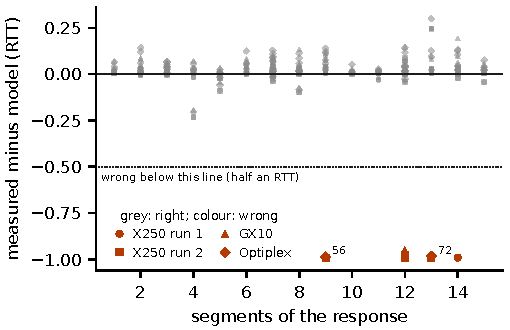
\includegraphics[width=0.62\textwidth]{fig_cells_map}
\caption{Error of the model in round trips against the segments of the response, one mark per design point and run.}
\label{fig:cellsmap}
\end{figure}

The model is wrong on \GnineCellsWrongXOne\ design points of the first X250 run, \GnineCellsWrongXTwo\ of its repeat, \GnineCellsWrongGx\ on the GX10, \GnineCellsWrongOp\ on the OptiPlex and \GnineCellsWrongNine\ on the i9, and \GnineCellsEvery\ design points (56 and 72) are wrong on every run. Every wrong design point is a round trip faster than predicted (Figure~\ref{fig:cellsmap}: all lie at $-1$~RTT, with responses of \GnineRespLo\ to \GnineRespHi\ segments). The other failing design points fail on only some machines: criterion A2 (at least four of the five design points wrong in the first X250 run are also wrong on the second machine) is met on the GX10 and the i9 but not on the OptiPlex, and V1 (the same test on the X250 again) is met. The registered rule therefore leads us to conclude that where the model fails depends partly on the machine. This fits a server window that differs between machines; the section on the server's window in the random design points, above, measures it. The ticket tests of Tests 16 and 18 are met on both machines (\GtwelveRepMet\ of \GtwelveRepK\ criteria).

\emph{Replications on the GX10 and the i9, November 25 and 26, 2026.} Criteria were registered before the runs and left unchanged (\texttt{results/g9\_gx10\_design.md}, \texttt{results/i9\_replication\_design.md}; written after the results of these tests on other machines had been seen). Tests 1 to 5 (Test 30) met G1 to G4 on both machines: rule~(1) was wrong on none of the 28 client-window design points and the loosened rule on 4; of the 10 design points where the ticket models differ, the separate-ticket model was wrong on none and the coalesced-ticket model on all; over all 80 ticket design points the separate-ticket model was wrong on \RoneGxEarly\ (GX10) and \RoneIEarly\ (i9), against \RoneXEarly\ on the X250. On the i9, the random design points (Test 28) met A1 to A4: wrong on design points 32, 56, 66 and 72, all of them wrong in the first X250 run, each one round trip too slow in the model. The new ticket design points (Test 16) met K1 to K4 at both RTTs, with the separate-ticket model wrong on one design point (RTT 200\ms, ML-DSA-65, response of 14 segments); delayed ACKs (Test 18) met D1 to D5. Under BBR (Test 17) B1 to B5 were met: the model with window $w_0+n$ was wrong on none of the client-window design points and rule~(1) on all 10 discriminating ones; the BBR ticket model was wrong on 3 of 41 design points and the model of the paper on 19 of the 21 where they differ. On plain TCP, the BBR and \texttt{fq} test (Test 15) met all of Q1 to Q5 on the i9, with the same median window as on the X250 at every size of every configuration (including Cubic with \texttt{fq} at 40 segments, 48 against 50 for rule~(1)). Under loss (Test 19) L1 to L3 were met, L1 only just: \GsixIWithin\ of 30 design points within six points of $(1-p)^n$, where at least 24 are required and the X250 had \GsixWithin; without a retransmission, \GsixINoRetxOk\ of \GsixINoRetxN\ connections had the window of rule~(1), and every design point off by more than six points lies above the prediction (\texttt{results/g16\_i9\_cells.txt}). That completes the replications registered for the i9. The background-load test (Test 24) we did not run on this shared machine.

\emph{Kernel results on the GX10 (Section~7.1 of the paper).} Most ticket results carry over from the X250 to the GX10. The state test (the paper's slow-start-condition test) always holds. Without a ticket the response burst stays within ten segments in all \ArmNoTktCells\ design points; with it, the burst changes in \ArmTktChangeW\ of them on both GX10 kernels and in \NtkEffectW\ on the X250. The two queueing explanations also fail here: on the GX10, \ArmBkSixFourteen\% and \ArmBkSevenZero\% of ticket ACKs are processed from the socket backlog (\BkIPct\% on the X250), and only \ArmLateSixFourteen\ of \ArmLateNSixFourteen\ and \ArmLateSevenZero\ of \ArmLateNSevenZero\ are processed after the write returned (\HALate\ of \HN\ on the X250). The first formula for the burst (P2), which Section~6 of the paper reports as failed, meets its criterion on the GX10 (\ArmBurstSixFourteen\% and \ArmBurstSevenZero\%) but not on the X250 (\StPTwoPct\%). The criterion that the \RaceThr\ms timing rule agree with the kernel's state near the threshold fails on both (\ArmThrSixFourteen\% and \ArmThrSevenZero\% on the GX10, \StPThreePct\% on the X250). Table~\ref{tab:repl} gives the plain-TCP match at MTU 9\,000 on every kernel, the state test, the no-ticket design points and the share of ticket ACKs processed from the socket backlog.

\begin{table}[h]
\caption{Replication on other kernels and CPUs.}
\label{tab:repl}
\centering\footnotesize\setlength{\tabcolsep}{3pt}
\begin{tabular*}{0.75\textwidth}{@{\extracolsep{\fill}}lcccc@{}}
\toprule
Platform, kernel & MTU 9\,000 & state & no ticket & backlog\\
\midrule
X250, 6.8 / 6.14 / 6.17 & \MtuISixEight\ / \MtuISixFourteen\ / \MtuISixSeventeen\% & -- & -- & --\\
X250, 7.0 & \MtuISevenZero\% & \StPOneRight/\StPOneN & \NtkCells/\NtkCells & \BkIPct\%\\
i9, 7.0.0-42 (2 runs) & \MtuNineI\% & -- & -- & --\\
GX10, 6.14 & \MtuArmSixFourteen\% & \ArmStateSixFourteen/\ArmStateSixFourteen & \ArmNoTktOk/\ArmNoTktCells & \ArmBkSixFourteen\%\\
GX10, 7.0 & \MtuArmSevenZero\% & \ArmStateSevenZero/\ArmStateSevenZero & \ArmNoTktOk/\ArmNoTktCells & \ArmBkSevenZero\%\\
\bottomrule
\end{tabular*}
\end{table}

\section*{Releases, controllers, load, and tails (Section~7.2)}
\emph{The ticket code across releases (Section~7.2).} The server's state transition after the client's Finished, the flush after ticket construction, and the construction itself are textually identical in OpenSSL 3.5.4, 3.5.9, and 3.6.5. Version 4.1.0 keeps the same order, although it adds DTLS~1.3 acknowledgments and moves the check of whether to send a ticket into the transition.

\emph{Why the Go model was wrong (Section~7.2).} All \GoWrongSuiteN\ wrong Go design points of the two tests are ML-DSA-87, each a round trip faster than predicted. A packet capture tells the story. The server's first flight (\GoChMlEightSeven\ segments) exceeds its window of ten, and the client sends its Finished and request without waiting for the tail of that flight, which holds the end of the ticket. A pipelined variant that no longer waits for the tail, devised after seeing the data, leaves \GoPostAfter\ of the \GoPostBefore\ design points wrong. We then registered the predictions of both models for \GeighteenN\ new ML-DSA-87 design points (RTT 30, 50 and 200\,ms, requests of 302 to 19\,460\,B, responses of 3 to 12 segments) and \GeighteenCtlN\ ML-DSA-65 controls whose first flight fits the window (Test 23). The pipelined variant was wrong on \GeighteenWrongPip\ of the new design points and the original on all \GeighteenWrongGo; all four criteria were met.

\emph{Detailed counts (Section~7.2).} \emph{Releases (Test~13).} Full handshakes agree with 3.5.4 in \OvTwoSame, \OvThreeSame\ and \OvFourSame\ of \OvTwoAll\ configurations for 3.5.9, 3.6.5 and 4.1.0, and the rest differ by at most one segment. In the repeated design points rule~(1) was wrong on \GxFourCWrong\ of the \CN\ client-window design points, the loosened rule on \GxFourCLoose, the separate-ticket model on \GxFourDisEarly\ and the coalesced-ticket model on \GxFourDisJoined\ of the \DDiff\ discriminating design points. \emph{Plain TCP (Test~15).} Under BBR rule~(1) is wrong for all \GelBbrWrongW\ sizes $n\le\GelBbrMax$, and a burst takes up to \GelBbrBurstMax\ms longer than on the baseline, pacing that the model leaves out. \emph{BBR ticket tests (Test~17).} Of the \GfBbrDN\ ticket-timing design points the BBR model was wrong on \GfBbrDWrong, and the model of the paper on \GfBbrRenoWrong\ of the \GfBbrDDiff\ design points where they differ; on \GfMidNW\ of those design points the measurement lies \GfMidAbove\ms above BBR's prediction and \GfMidBelow\ms below Reno's. \emph{Delayed acknowledgments (Test~18).} Rule~(1) was wrong on \GfDelCWrong\ of \GfDelCN\ design points and the separate-ticket model on \GfDelEarlyAll\ of \GfDelDN. \emph{New Go design points (Test~23).} The largest error of the pipelined variant was \GeighteenMaxErr\ms on the new design points and \GeighteenCtlErr\ms on the controls.

\emph{Background load (Section~7.2).} Test 24 used four levels: L0, no load (control); L1 cross traffic on the link (UDP at 40\,Mbit/s and ten TCP connections of 2\,Mbit/s each; \GseventeenUdp\ and \GseventeenTcp\,Mbit/s were achieved, about 58\,\% of the 100\,Mbit/s link); L2 a busy loop on every CPU, including those of the client and server probes; L3 both. The \GseventeenCells\ design points are the client-window and ticket-timing design points of Test 18 ($n=30$, predictions unchanged). At every level the model was wrong on \GseventeenWrongMax\ of the \GseventeenCells\ design points and the coalesced-ticket model on \GseventeenJoinedMin\ of the \GseventeenDisc\ discriminating design points; the load moved the excess of a design point by at most \GseventeenShiftMax\,ms against no load. One fixed traffic mix on one bottleneck and a busy loop are no substitute for production traffic or load.

\emph{Tails (Section~7.2).} Table~\ref{tab:tails} gives the six design points measured with $n=1\,000$ transactions each (Test 22). Each distribution has a single narrow peak, with a maximum at most 2.5\,ms above the median and no transaction more than 20\,ms above it, so no tail hides an extra round trip. Still, six design points are a small sample of the design space.

\begin{table}[h]
\caption{Latency of the six design points with $n=1\,000$ (ms; the last column is the share of transactions above the median by more than 20\,ms, in \%).}
\label{tab:tails}
\centering\footnotesize\setlength{\tabcolsep}{4pt}
\begin{tabular}{@{}llrrrrrr@{}}
\toprule
Suite & Request / response (B) & $n$ & Median & P99 & P99.9 & Max & Above 20\,ms\\
\midrule
\TailRows
\bottomrule
\end{tabular}
\end{table}

\section*{A third library: GnuTLS (Section~7.2)}
We then turned to GnuTLS~3.8.14, another TLS~1.3 implementation, built with leancrypto to provide ML-DSA and hybrid ML-KEM groups (the distribution's 3.8.3 has neither). According to its source (read on November 19, 2026; \texttt{results/tls\_libs\_ticket\_source\_audit\_20261119.md}, which also records the reading of wolfSSL~5.9.4, not measured) it writes tickets after the client's Finished, as OpenSSL does, but sends \emph{two} in one flush, each containing the client's certificate list. A loopback calibration of its writes (\texttt{results/gnutls\_calibration.json}) confirms this: the tickets are one write of 2\,626, 9\,826, 12\,898 and 16\,802 bytes for ECDSA-P256 and ML-DSA-44, -65 and -87 (2, 7, 9 and 12 segments), twice the size of OpenSSL's. GnuTLS offers no pure ML-KEM in TLS, so we use the hybrids X25519MLKEM768 and SECP384R1-MLKEM1024 (key shares 32 and 97 bytes larger); the model uses the sizes measured in calibration. Our probe lets the application send 0 to 4 tickets (\texttt{gnutls\_session\_ticket\_send}), which allows the key experiment: the amount of ticket data varies while the suite, ClientHello, client window, and request stay fixed.

\emph{Design (fixed on November 22, 2026, commit 9fc59f9, before the measurement).} The model was unchanged and nothing was fitted; predictions depend only on the calibration and \texttt{pqc\_sim.py}. All runs used resumed TLS~1.3 with mutual authentication (depth 1, RTT 100\,ms, 100\,Mbit/s, MTU 1\,500, initial window 10, $n=30$, CPU clock fixed) on the X250 and the GX10. Stage T, the main experiment, covers 100 design points (ML-DSA-44 and -65; 0 to 4 tickets, that is, 0 to 14 and 0 to 18 segments; responses of 4 to 22 segments; request 302\,B), each compared with two predictions: \emph{inflight}, the paper's model, in which the tickets share the server's window of ten with the response; and \emph{acked}, in which the tickets are acknowledged before the response is sent, so that the response alone uses the window given by rule~(1) for the ticket flight. The two differ by half an RTT in 57 design points. Stage C has 32 client-window design points (rule~(1) against the rule loosened by two segments and textbook slow start). Stage D has 85 ticket-position design points (separate-ticket against coalesced-ticket model; the two differ in 35). Stage R has 40 randomly drawn design points (seed 20261123; design space of the first random draw; depth 1). Stage O repeats 20 design points of D with OpenSSL~3.5 in the same session to separate library effects from session effects. Our goal here was to understand what sets the server's window, not to pass or fail. Each count has a band, derived from the OpenSSL and Go counts in the paper, within which a library behaving like those references would fall with 95\% probability; a count above its band calls for diagnosis.

\begin{table}[h]
\caption{GnuTLS~3.8.14 on the GX10 and the X250 (\texttt{results/g23\_report.txt}).}
\label{tab:gtls}
\centering\footnotesize\setlength{\tabcolsep}{4pt}
\begin{tabular}{@{}lcrr@{}}
\toprule
Count & Band & GX10 & X250\\
\midrule
C: rule~(1) wrong, of \GtlsACN\ design points & 0--2 & \GtlsACWrong & \GtlsXCWrong\\
C: loosened rule / textbook slow start refuted, of \GtlsAAltCN\ / \GtlsATextN\ & & \GtlsAAltCWrong\ / \GtlsATextWrong & \GtlsXAltCWrong\ / \GtlsXTextWrong\\
D: separate-ticket model wrong where it differs from the coalesced, of \GtlsADisN\ & 0--3 & \GtlsADisWrong & \GtlsXDisWrong\\
D: separate-ticket model wrong, of \GtlsADN\ & 0--14 & \GtlsADWrong & \GtlsXDWrong\\
R: model wrong, of \GtlsARN\ random design points & 0--3 & \GtlsARWrong & \GtlsXRWrong\\
O: model wrong on OpenSSL in the same session, of \GtlsAON & 0--2 & \GtlsAOWrong & \GtlsXOWrong\\
C, D, R: model too fast by more than half an RTT & 0--1 & \GtlsAFast & \GtlsXFast\\
T: design points where the latency follows \emph{inflight} / \emph{acked} / either, of \GtlsATN & & \GtlsATInflight\ / \GtlsATAcked\ / \GtlsATBoth & \GtlsXTInflight\ / \GtlsXTAcked\ / \GtlsXTBoth\\
T: series (of \GtlsATSeries) where the extra round trip appears at the model's response size & & \GtlsATSeriesMatch & \GtlsXTSeriesMatch\\
Wrong design points in C, D, R (all too slow, by \GtlsAMinSlow\ to \GtlsAMaxSlow\,ms on the GX10) & & \GtlsAWrong & \GtlsXWrong\\
\quad of them with a request of more than 13\,KB & & \GtlsAWrongBigReq & \GtlsXWrongBigReq\\
\bottomrule
\end{tabular}
\end{table}

\emph{What the data show.} (i)~With a small request, ticket size does not set the server's window: in stage T, latency follows the model on every design point where the two predictions differ, for 0 to 18 segments of ticket data, and no design point follows the window grown by rule~(1). (ii)~Parts of the model hold on a third library: rule~(1) on its ClientHello and the separate-ticket position (no wrong design point where the two ticket models differ); the OpenSSL control in the same session shows that the sessions were sound. The random design points, however, fall outside their band. (iii)~As in the paper, the errors are one-sided, here in the direction fixed beforehand (band 0--1 for ``too fast'', Table~\ref{tab:gtls}): in none of the \GtlsFastCellRuns\ design-point runs of C, D, and R on the two machines was the model too fast. (iv)~On both machines the wrong counts on the random design points exceed the band (\GtlsARWrong\ and \GtlsXRWrong\ against 0--3). Every wrong design point is predicted too slow and has a request larger than 13\,KB, which needs another round trip, so the ticket is acknowledged before the response leaves; in that case the model leaves the server's window at ten. OpenSSL behaves similarly: over the five runs of the first random draw, \DomLargeWrong\ of the \DomWrongTotal\ wrong design-point runs have a request of more than 13\,KB; \DomLargePct\,\% of the \DomLargeN\ design-point runs with such a request are wrong, \DomRestPct\,\% of the \DomRestN\ with a smaller one (the wrong ones among these include the ticket-size error of Section~7.2 of the paper). Request size marks this case; we have not shown that it is the cause. (v)~The machine does not decide the outcome: of the \GtlsBothCells\ design points measured on both, the excess differs by more than half an RTT on \GtlsBothDiffer, and the \GtlsSharedWrong\ wrong design points of the GX10 are wrong on the X250 too (it has two more). At the resolution of this test, then, we find no support for the idea that machine-dependent microsecond orderings change the latency of these design points. This does not contradict the kernel measurements in ``The server's window, acknowledgment by acknowledgment,'' which take the processing times as measured and say nothing about how they differ between machines.

\emph{Exploratory: a partial rule.} Could a simple rule account for the wrong design points? We formulated one after seeing the GX10 data and committed its X250 predictions, for the same design points, before looking at the X250 data. In case (iv), the server's window might equal rule~(1) applied to the ticket flight (14, 18 and 22 segments for the three ML-DSA suites of GnuTLS): \texttt{gnutls\_explore.py}. On the GX10 it makes \GtlsAHackDFixed\ of the \GtlsADWrong\ wrong design points of D and \GtlsAHackRFixed\ of the \GtlsARWrong\ of R right and breaks \GtlsAHackDBroke\ design points of D (ML-DSA-87, responses of 19 to 21 segments, where the measured window is about 18, not 22); on the X250 it fixes \GtlsXHackDFixed\ and \GtlsXHackRFixed\ and breaks \GtlsXHackDBroke\ and \GtlsXHackRBroke. On the random draws of OpenSSL it changes no design point, because tickets of about five segments give a window of ten by rule~(1). At best, then, the rule applies to large tickets. What sets the window after an acknowledged 12-segment ticket, and in the OpenSSL design points with small tickets, remains open.

\emph{Limits of this test.} It uses depth-1 chains, hybrid key exchange in place of ML-KEM, one resumption per transaction, and an emulated link; the number of tickets is set through the application's call, not by patching the library. Stage T has one request size (302\,B), so the response leaves right after the Finished. It ran on two machines; they agree on all but two of \GtlsBothCells\ design points, so we skipped the planned X250 repeat. Other users loaded the GX10 (load 0.4 to 1.0). The analysis is \texttt{testbed/analyze\_g23.py} and \texttt{testbed/g23\_report.py}, the data are in the archive (runs 20261122-141612-gx10-g23-gx10 and 20261122-145057-X250-g23-X250).

\section*{A second random draw (Section~7.2)}
One draw can mislead. So, after fixing the paper's predictions, we drew another 100 design points at random from the design space of Test 20 (new seed, no design point reused) and measured them on the X250 and the GX10, with the model's predictions written down before any measurement (\texttt{results/g22\_round2\_predictions.md}). The model was wrong by more than half an RTT on \GttXRWrong\ of the \GttXRN\ design points on the X250 (mean absolute error \GttXRMae\,ms; \GttXRTwo\ design points within 2\,ms) and on \GttARWrong\ on the GX10 (\GttARMae\,ms; \GttARTwo\ design points within 2\,ms, the rest a constant offset of about 3\,ms of that machine). For comparison, on the first and second draws the model was wrong on \GnineCellsWrongXOne\ and \GttXRWrong\ of 100 design points on the X250 and on \GnineCellsWrongGx\ and \GttARWrong\ on the GX10. We also measured \GttXFN\ design points chosen on purpose: those for which an alternative model of the ticket ACKs (not part of this paper) predicted a faster response. The paper's model was wrong on \GttXFWrong\ of them on the X250 and on \GttAFWrong\ on the GX10, as expected where the server's window after the ticket exceeds ten, which the model does not predict. All \GttDirSlow\ wrong design-point runs of this draw (of \GttDirRuns) are too slow and none is too fast; the largest underestimate is \GttDirMaxX\,ms on the X250 and \GttDirMaxA\,ms on the GX10. Because the criteria registered for this draw concerned the alternative model, the results for the paper's model are reported, not tested. As in the first draw, the failing region depends on the machine. To see how much of this is noise, we repeated the X250 measurement once, with the same design points and predictions, declared in advance as a run to estimate the noise floor. The model was then wrong on \GttXRunTwoWrong\ of the 100 design points (mean absolute error \GttXRunTwoMae\,ms) instead of \GttXRWrong, and the measured excess of \GttXNoise\ of the 130 design points differs between the two runs by more than half an RTT. The number of wrong design points in a run of 100 therefore varies by a few design points by chance. The repeat, too, had no design point where the model was too fast.

\section*{Smaller errors and earlier runs (Section~7.2)}
\emph{The ticket-size error (Section~7.2).} The one discriminating design point of the random draw that the separate-ticket model got wrong is an ECDSA-P256 design point with a small request, which the coalesced-ticket model got right. The ticket of the model is \TktDiffLo\ to \TktDiffHi\ bytes larger than the one on the wire (\TktModelEc\ against \TktWireEc\ bytes for ECDSA-P256), which at the MSS of that design point turns one segment into two and pushes ticket and response past the window of ten. With the measured size that prediction changes from \TktCellOld\ to \TktCellNew\,ms, and no other prediction of the \GnineN\ design points changes by more than 1\,ms. We caught this error only afterward, so we tested the correction with predictions fixed first (Test 26): remeasured with $n=200$, the design point gave \GnineBRepeat\,ms, as before; the model with the measured ticket size was right on all six design points of that family (responses of 9\,500 to 12\,400\,B), the earlier model on none of the \GnineBDisc\ design points where the two differ, and the step from three to four round trips lies between \GnineBLo\ and \GnineBHi\,B.

\emph{Design points off by a few milliseconds (Section~7.2).} The ten design points of the random draw that are within half an RTT but off by more than 2\,ms are all at 10\,Mbit/s, with errors of \GnineOffLo\ to \GnineOffHi\,ms (Table~\ref{tab:offcells}; positive: the model is slower than the measurement). They go both ways and stay far below an RTT; we did not investigate them. At the millisecond level, then, the model's errors are not one-sided, which is why the direction counts above include only errors larger than half an RTT.

\begin{table}[h]
\caption{The ten design points of the random draw that are off by more than 2\,ms but by less than half an RTT (first X250 run).}
\label{tab:offcells}
\centering\footnotesize\setlength{\tabcolsep}{4pt}
\begin{tabular}{@{}rlrrrrr@{}}
\toprule
Design point & Suite & RTT (ms) & Rate (Mbit/s) & MTU & Request / response (B) & Error (ms)\\
\midrule
\OffRows
\bottomrule
\end{tabular}
\end{table}

\emph{Runs that preceded the reported ones.} The physical-link test (Test 25) began with a smoke run ($n=3$); its plain-TCP part was complete and gave the same result, but we do not use it. The first Go run (Test 14) lacked the ECDSA-P256 set, which we measured separately on the same machine; criteria H1 to H5 use the merged runs, with predictions and criteria unchanged. We repeated the ticket ACK traces on one clock only after reading the first traces, and we keep and report both sets.

\section*{What remains open}
\emph{Established.} (i)~Without the ticket, the burst stays within ten segments. (ii)~\texttt{tcp\_slow\_start} runs exactly when the kernel's test holds, and each ACK updates the window by the slow-start rule (\RbEvOk\ of \RbEvN\ window events). (iii)~The burst formula fixed on a pilot holds on the X250 test (\RbTestTxOk\ of \RbTestTxN\ transactions). (iv)~Late ACKs reach the server's input queue after the response write has returned (median \HEnqMed\,\textmu s) and wait there a median of \HWaitMed\,\textmu s to be processed, on the same CPU.

\emph{Refuted or not supported.} (i)~A larger client window as the cause of the model's error on the request flight (the loosened rule, Table~2 of the paper). (ii)~A ticket written together with the response (the coalesced-ticket model). (iii)~Socket ownership or the softirq queue as the cause of late ACKs (criteria G1a, G1b, H1a, H1b). (iv)~Late ACKs preceding the response (a capture timestamp artifact). (v)~A single timing threshold for all machines and CPU clock settings.

\emph{Not established.} One question stays open: we do not know why the ACKs are processed when they are, and nothing here predicts those times from network parameters. Because neither socket ownership nor the softirq queue accounts for the delay of the late ACKs, we infer that it arises before the server's input queue, but we have not located it (the client, its \texttt{netem} qdisc, or the virtual link), nor traced it over the cable of Test~25. In the OpenSSL design points with small tickets that the model gets wrong (a request that needs another round trip, so that the ticket is acknowledged before the response leaves), the fast transactions have a larger server window (Test~31), but we do not know why the window grows in some transactions and not in others. We also cannot explain the corresponding wrong design points of GnuTLS, where we did not measure the window.

\emph{Next measurements.} (i)~Timestamps for each ACK at the server's NIC, driver, and receive path, to locate the \HEnqMed\,\textmu s delay. (ii)~The same ticket design points, with the same probes, on a physical path whose delay is not emulated. (iii)~What decides, on each machine, whether the ACKs of an already acknowledged ticket have enlarged the server's window, which rule~(1) does not predict. (iv)~Tails in more design points near the window boundary and with concurrent connections.

\section*{Sources of the numbers}
Table~\ref{tab:repro} lists the script and output behind each number. Scripts are in \texttt{Measurements/testbed/} and outputs in \texttt{Measurements/testbed/results/}. The script \texttt{make\_assets\_short.py} (in \texttt{paper2\_short/Latex/}) reads the outputs and writes the generated numbers of the paper and this supplement to \texttt{numbers\_short.tex}. The raw traces are on Zenodo in three parts: the ticket tests of November 1 and 2, Tests 6 to 12 (doi:\allowbreak10.5281/\allowbreak zenodo.\allowbreak24384873); the clock-safe repeat of November 21 on the x86 machines (doi:\allowbreak10.5281/\allowbreak zenodo.\allowbreak24419058); and the later runs, namely the repeat on the GX10 (November 21), the exploratory runs and the four rounds of the intervention (November 22 and 23), Test 31 (November 25), and the repeat and the fourth round on the i9 (November 26) (doi:\allowbreak10.5281/\allowbreak zenodo.\allowbreak24552433). For the first part, \texttt{tools/raw\_traces.sh verify DIR} reruns the analyses on the traces unpacked in \texttt{DIR} and compares the results with the archived outputs. Table~\ref{tab:repro} lists the scripts that produce the numbers taken from the other parts. From the published kernel traces, the lines that report connections outside the testbed are removed and the names of other processes are replaced by \texttt{other} (\texttt{tools/filter\_kernel\_traces.py}); the analyses give the same output on the filtered traces.

\begin{table}[h]
\caption{Scripts and outputs.}
\label{tab:repro}
\centering\footnotesize\setlength{\tabcolsep}{4pt}
\begin{tabular}{@{}p{0.40\textwidth}p{0.25\textwidth}p{0.28\textwidth}@{}}
\toprule
Number & Script & Output\\
\midrule
Captures: \RaceN\ transactions, \RaceBeforePct\%, \RaceRight\ of \RaceMlN & \texttt{analyze\_ticket\_race.py} & \texttt{ticket\_race.csv}, \texttt{wp6\_analysis\_race.txt}\\
Sweep: \RaceTwoRight\ of \RaceTwoScored, \RaceTwoOosRight\ of \RaceTwoOosN & \texttt{analyze\_race2.py} & \texttt{wp6\_analysis\_race2.txt}\\
Threshold table & \texttt{threshold\_sweep.py} & \texttt{wp6\_analysis\_threshold.txt}\\
Function trace: \KerRight\ of \KerN & \texttt{analyze\_ftrace.py} & \texttt{wp6\_analysis\_kernel.txt}\\
State trace: \StN, P1--P3 & \texttt{analyze\_state.py} & \texttt{wp6\_analysis\_state.txt}, \texttt{ticket\_state.csv}\\
Backlog: \BkN & \texttt{analyze\_backlog.py}, \texttt{analyze\_backlog\_posthoc.py} & \texttt{wp6\_analysis\_backlog.txt}, \texttt{wp6\_analysis\_backlog\_posthoc.txt}\\
Softirq: \HN, \HALate, \HEnqMed\,\textmu s & \texttt{analyze\_softirq.py}, \texttt{analyze\_softirq\_posthoc.py} & \texttt{wp6\_analysis\_softirq.txt}, \texttt{wp6\_analysis\_softirq\_posthoc.txt}\\
No ticket: \NtkCells\ design points, $p=\SignNtkP$ & \texttt{analyze\_notkt.py} & \texttt{wp6\_analysis\_notkt.txt}\\
Clocks: \ClkN\ acknowledgments & \texttt{analyze\_clock\_check.py} & \texttt{wp6\_clock\_check.txt}\\
Other machines: A1--A4, V1--V3, K1--K4, D1--D5 & \texttt{analyze\_\allowbreak g19\_\allowbreak arm.py}, \texttt{analyze\_\allowbreak g12.py}, \texttt{analyze\_\allowbreak g14.py} & \texttt{g19\_\allowbreak *\_\allowbreak analysis.txt}, \texttt{g12\_\allowbreak *\_\allowbreak analysis.txt}, \texttt{g14\_\allowbreak *\_\allowbreak analysis\_\allowbreak *.txt}\\
Plain TCP on the i9 (Tests 15 and 19) & \texttt{analyze\_\allowbreak g11.py}, \texttt{analyze\_\allowbreak g16.py}, \texttt{analyze\_\allowbreak g16\_\allowbreak cells.py} & \texttt{g11\_\allowbreak i9\_\allowbreak analysis.txt}, \texttt{g16\_\allowbreak i9\_\allowbreak analysis.txt}, \texttt{g16\_\allowbreak i9\_\allowbreak cells.txt}\\
Tests 1--5 on other machines; i9 repeats of the clock test and the fourth round & \texttt{analyze\_\allowbreak g9.py}, \texttt{analyze\_\allowbreak clock\_\allowbreak repeat.py}, \texttt{r3d.py} & \texttt{g9\_\allowbreak *\_\allowbreak analysis.txt}, \texttt{wp6\_\allowbreak clock\_\allowbreak repeat\_\allowbreak i9\_\allowbreak analysis.txt}, \texttt{r3d\_\allowbreak i9\_\allowbreak test.txt}\\
Server window in random design points (Table~\ref{tab:gtf}) & \texttt{g24\_\allowbreak predict.py}, \texttt{analyze\_\allowbreak g24.py}, \texttt{analyze\_\allowbreak g24\_\allowbreak posthoc.py} & \texttt{g24\_\allowbreak *\_\allowbreak analysis.txt}, \texttt{g24\_\allowbreak *\_\allowbreak posthoc.txt}, \texttt{g24\_\allowbreak *\_\allowbreak posthoc\_\allowbreak points.csv}\\
Clock-safe repeat (Table~\ref{tab:clock}) & \texttt{clock\_sync.py}, \texttt{ticket\_\allowbreak xmit.bt}, \texttt{analyze\_\allowbreak clock\_\allowbreak repeat.py}, \texttt{compare\_\allowbreak race\_\allowbreak bursts.py} & \texttt{wp6\_clock\_\allowbreak repeat\_\allowbreak tuned\_\allowbreak analysis.txt}, \texttt{wp6\_clock\_\allowbreak repeat\_\allowbreak analysis.txt}, \texttt{wp6\_clock\_\allowbreak repeat\_\allowbreak bursts.txt}, \texttt{wp6\_\allowbreak clock\_\allowbreak repeat\_\allowbreak gx10\_\allowbreak analysis.txt}, \texttt{wp6\_\allowbreak k7\_\allowbreak points\_\allowbreak *.csv} (Figure~\ref{fig:k7})\\
Design points of the random design (Figure~\ref{fig:cellsmap}) & \texttt{make\_\allowbreak assets\_\allowbreak short.py} & \texttt{g19\_\allowbreak *\_\allowbreak cells.txt}\\
Second random draw: \GttXRN\ random design points per machine & \texttt{g22\_\allowbreak predict.py}, \texttt{analyze\_\allowbreak g22.py} & \texttt{g22\_\allowbreak *\_\allowbreak analysis.txt}, \texttt{g22\_\allowbreak predictions.csv}\\
Third library, GnuTLS (Table~\ref{tab:gtls}) & \texttt{gnutls\_\allowbreak calibrate.py}, \texttt{gnutls\_\allowbreak predict.py}, \texttt{analyze\_\allowbreak g23.py}, \texttt{g23\_\allowbreak report.py} & \texttt{g23\_\allowbreak report.txt}, \texttt{g23\_\allowbreak gx10\_\allowbreak analysis.txt}, \texttt{g23\_\allowbreak x250\_\allowbreak analysis.txt}\\
The window ACK by ACK (Table~\ref{tab:rbtwo}) & \texttt{analyze\_\allowbreak r3.py}, \texttt{r3b\_\allowbreak analyze.py}, \texttt{r3b\_\allowbreak thresholds.py}, \texttt{r3b\_\allowbreak test.py}, \texttt{r3b\_\allowbreak report.py} & \texttt{r3b\_\allowbreak report.txt}, \texttt{r3b\_\allowbreak thresholds.md}, \texttt{r3\_\allowbreak gx10\_\allowbreak findings.md}\\
The write delayed (Tables~\ref{tab:rcthree} and~\ref{tab:rdfour}) & \texttt{r3c.py}, \texttt{r3c\_report.py}, \texttt{r3d.py}, \texttt{r3d\_report.py} & \texttt{r3c\_report.txt}, \texttt{r3d\_report.txt}\\
Direction of the errors (Table~\ref{tab:dir}) & \texttt{one\_\allowbreak sided\_\allowbreak errors.py} & \texttt{one\_\allowbreak sided\_\allowbreak errors.txt}\\
Segment counts of Dubetskyy and Cano (Section~5 of the paper) & \texttt{analyze\_\allowbreak dubetskyy\_\allowbreak segments.py} & \texttt{dubetskyy\_\allowbreak segments\_\allowbreak 20261116.txt}\\
OpenSSL ticket code across releases (Section~7.2 of the paper) & \texttt{audit\_\allowbreak ossl\_\allowbreak ticket\_\allowbreak path.py} & \texttt{ossl\_\allowbreak ticket\_\allowbreak path\_\allowbreak audit.txt}\\
Model components (Table~\ref{tab:ablation}) & \texttt{analyze\_l1\_model\_comparison.py} & \texttt{l1\_model\_comparison.csv}, \texttt{.txt}\\
\bottomrule
\end{tabular}
\end{table}

\end{document}
